\documentclass[12pt]{paper}
\usepackage[margin=1in]{geometry}
\usepackage{float}
\usepackage{natbib}
\bibliographystyle{apsr}
\usepackage{graphicx}
\graphicspath{ {../fig/} }
\usepackage{setspace}
\usepackage[super]{nth}
\usepackage{booktabs}
\usepackage{subfig}
\usepackage{makecell}
\usepackage{amsmath}
\usepackage{dcolumn}
%\usepackage{authblk}
\usepackage{hyperref}
\usepackage{wrapfig}
\usepackage{amsmath}
\usepackage{adjustbox}
\usepackage{hanging}
%\usepackage{etoolbox}
%\AtBeginEnvironment{quote}{\singlespacing\small}

\newlength{\cslhangindent}
\setlength{\cslhangindent}{1.5em}
\newenvironment{cslreferences}%
{\setlength{\parindent}{0pt}%
	\everypar{\setlength{\hangindent}{\cslhangindent}}\ignorespaces}%
{\par}

\title{Symbolic Racism, Racial Resentment, and Sophistication Reconsidered}
\author{Sarah ``Dot" Warren}
\date{}

\begin{document}
\maketitle
%\thispagestyle{empty}
%\clearpage
%\setstretch{1}

\doublespacing
\section*{Introduction}
Despite the widespread belief that the United States is a ``post-racial" society, black Americans continue to experience disproportionate discrimination and violence when interacting with police \citep{knox_administrative_2020, zhao_note_2022}, healthcare workers \citep{flores_racial_2005, penner_reducing_2014}, and employers \citep{quillian_meta-analysis_2017, kang_whitened_2016}. Compounding these disadvantages is the fact that black Americans have long earned less and enjoyed less wealth \citep{shapiro_hidden_2004} than white Americans. Past work has shown that a critical component of whites' attitudes about black Americans is their beliefs about the underlying causes of poverty in the black community. Some whites believe the observed economic disparities arise out of individual qualities of dependence and laziness among black Americans. This is called ``individualistic attribution." Others whites, however, view racial disparities as functions of systemic racism, lack of opportunity, and the legacy of slavery and discrimination black Americans have faced for decades \citep{feagin_poverty_1972}.  This is called ``structuralist attribution."

Previously, \cite{gomez_rethinking_2006} demonstrated that political sophistication was a key cognitive mechanism for understanding \textit{how} and \textit{why} these different attributions are made, using data from the late 20th and early 21st Centuries. Specifically, they argue that political sophistication enables individuals to make abstract attributions, such as attributing the economic conditions of the black community to a complicated system of structural factors. In this paper, I take up where \cite{gomez_rethinking_2006} left off and reconsider the role of sophistication in structuralist attributions in the 21st Century. Specifically, I demonstrate that  while political sophisticates are less likely than non-sophisticates to make individualistic attributions, there is no longer a meaningful relationship between sophistication and structuralist attributions. I argue that this null relationship is a product of an information-saturated environment, in which those who are politically sophisticated need not have a great breadth or depth of political knowledge, as was once the case. Further, I demonstrate that racially salient events in the early 21st Century contributed to a wider awareness of structural and institutional bias against black Americans. Taken together, I argue that these factors have lowered the cognitive barrier once-thought necessary to make structuralist attributions. Using data from the 2012-2016 ANES, I estimate ordered probit models that provide evidence for these claims.

The rest of this paper proceeds as follows: Section I introduces the empirical background and theory behind heterogeneous attributions for the causes of poverty, specifically among black Americans. Section II introduces the data and my empirical approach, including relevant descriptive statistics. Section III presents the main findings and Section IV prevents relevant model diagnostics. Section V concludes.

\section{Background and Theory}
\cite{gomez_political_2001, gomez_rethinking_2006} articulate a theory of heterogeneous attribution in which sophisticates and non-sophisticates in the public leverage different information and cognitive processes when evaluating political phenomena. Political sophistication, or the breadth and depth of one's political knowledge, enables individuals to make broad and nuanced attributions about the underlying causes of political phenomena, including black poverty. Conversely, less sophisticated individuals tend to make proximal attributions. Sophisticates, therefore, are much more likely to make complex, structural attributions, while non-sophisticates are more likely to blame individuals for their own circumstances. It is therefore no surprise that, in their evaluation of the 1986 and 2000 American National Election Study's (ANES) symbolic racism items, low sophisticates almost exclusively make individualist attributions. In other words, a nontrivial proportion of low sophisticates may have been incorrectly labeled as having racial animus, when in fact their individualist attributions may not reflect true animus, but simply low sophistication and a cognitive inability to make higher-level attributions \citep{gomez_rethinking_2006}. In other words, these low sophisticates were to suddenly acquire a great deal of political information, making them politically sophisticated, we should expect, \textit{ceteris paribus}, their attributions to shift from individualistic to structural.

The question concerning this discussion is whether the 21st Century American public possesses different information about the connection between race, poverty, and political institutions than the 20th Century American public surveyed in Gomez and Wilson's 2006 study. Many racially significant events have occurred in the 21st Century, from the election of the first black President of the United States to the rise of the Black Lives Matter movement in 2014. Moreover, the public-facing dialogue about institutional racism and structural barriers to black American's economic well-being have increased dramatically in the 21st Century. For example, though the idea of reparations has been around since the Civil War, the debate moved to the national discourse in 2014 when journalist Ta-Nehisi Coates wrote “The Case for Reparations” for \textit{The Atlantic,} prompting a tidal wave of digital content surrounding the issue \citep{coates_case_2014}. Notable voices in the conversation included Antonio Moore and Yvette Carnell, co-founders of the American Descendants of Slavery (or ADOS) movement, who took to Twitter, YouTube, and public radio to make their case for reparations to combat decades of structural racism in the United States. In the 2020 Presidential elections, then-candidates Kamala Harris, Elizabeth Warren, Cory Booker, Julian Castro, and Marianne Williamson all supported reparations for black Americans and descendants of slaves \citep{lockhart_2020_2019}. The mere willingness of some Democratic candidates to say they support reparations reflects a shift from recent years; indeed, President Barack Obama did not endorse reparations or support creating a reparations program. Outside of electoral politics, students at Georgetown University made national headlines in April when they voted to create a reparations fund supporting the descendants of the 272 slaves once owned by the school \citep{hassan_georgetown_2019}.

%[GOOGLE TRENDS GRAPHIC HERE]
\begin{figure}[h!]
%	\centering
	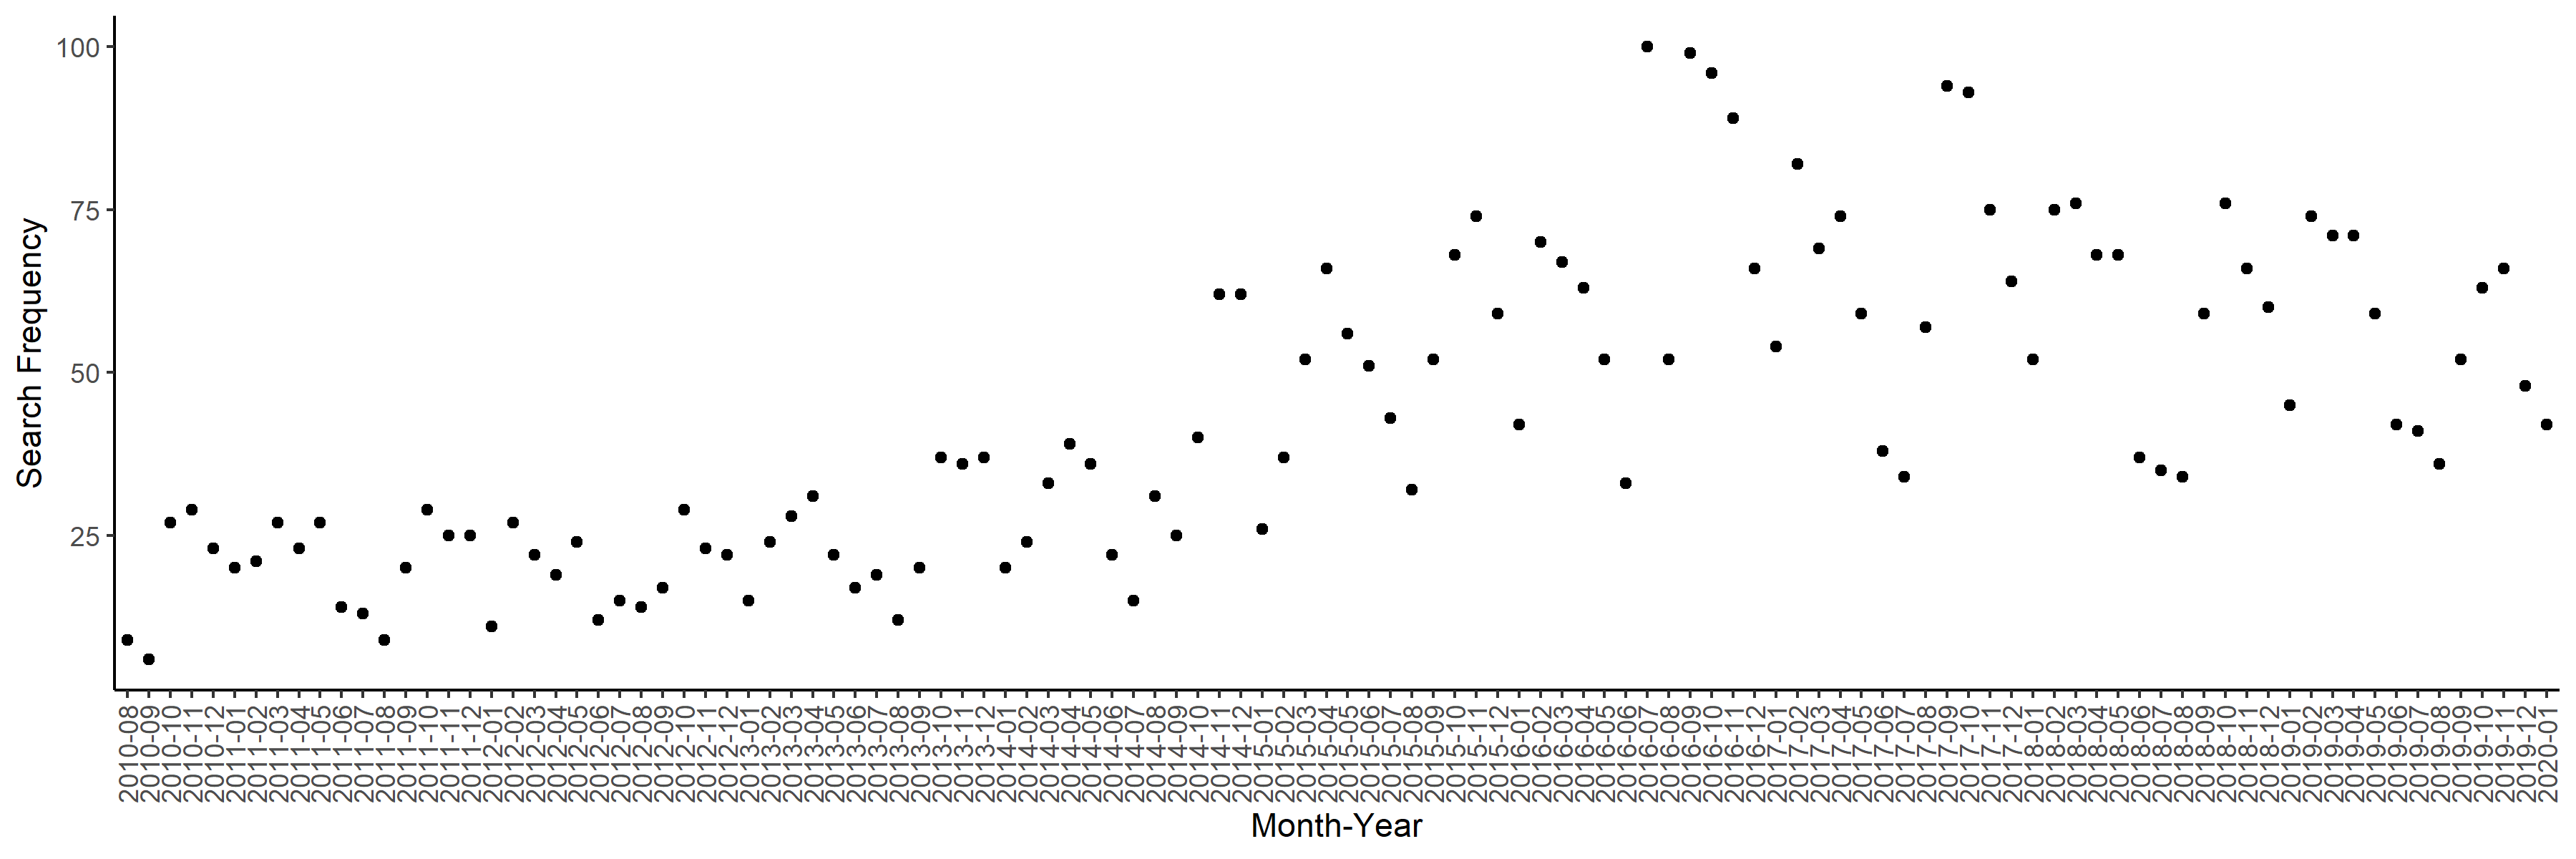
\includegraphics[scale=.55]{fig/google-trends.png}
	%{\singlespacing
	%	\parbox{0.78\textwidth}{\scriptsize%\vspace{-0.25cm}
	%		Notes: Explain the figure here
	%}}
	\caption{Google Search Trends for Topic: Institutional Racism}
	\label{trends}
\end{figure}

Irrespective of whether the increased public discourse moved public opinion on reparations, it has certainly increased awareness and curiosity about structural racism. Google trends show a steady increase in searches related to ``institutional racism" from 2010-2020, with a noticeable rise beginning in mid-2012. This suggests that an increasing number of people have recently been exposed to institutional racism as a possible explanation for the relatively lower socioeconomic status of black Americans. Additionally, the dissemination of this information in digital, accessible formats like \textit{The Atlantic}, social media, and presidential debates has made it more accessible to a wider population of Americans, even perhaps those with low political interest. Whereas institutional racism may have been a more academic argument in the late 20th Century, available only to those with the deepest and broadest wells of political knowledge, in the early 21st Century, it may be an accessible enough of an explanation for low-sophisticates to employ it when asked to consider the causes of black poverty.

Given this, I expect that political sophistication will no longer predict structural attributions. That is, holding all else constant at its mean, those who are high in political sophistication should be no more likely to attribute black poverty to structural causes than those low in political sophistication.

\section{Data and Method}
To test my hypothesis that sophistication no longer predicts distal attributions, I perform an analogous analysis to \cite{gomez_rethinking_2006} using data from the 2012 and 2016 ANES. However, there are some key differences in the 2012 and 2016 ANES batteries and the the 1986 and 2000 ANES surveys used in the original analysis. This section details the main variables included in the model and, if they differ from the original model specifications, the manner in which they differ.

\subsection{Dependent Variables}
To what or whom do whites attribute the cause of black poverty? Broadly, I am interested in two classes of outcomes: individual attributions and structural attributions. To measure both of these constructs, I use questions from the ANES Symbolic Racism Scale \citep{kinder_divided_1997}. These questions are constant across both the 2012 and 2016 ANES.

Two items on the symbolic racism scale clearly tap into individualistic attributions for racial economic disparities in American society. These questions attribute the economic plight of black Americans to personal qualities of laziness and individual failings. They are as follows: 

\begin{enumerate}
\item``Irish, Italians, Jews, and many other minorities
overcame prejudice and worked their way up. Blacks should do the same without any special favors.”

\item``It’s really a matter of some people not trying
hard enough; if blacks would only try harder they
could be just as well off as whites.”
\end{enumerate}

The other two items on the symbolic racism scale tap into structuralist attributions for racial economic disparities. Instead of blaming black Americans for having or failing to have certain personal qualities, these explanation attribute the locus of causality outside of the individuals involved, blaming institutions and systems rather than people. They are as follows: 

\begin{enumerate}
	\item``Over the past few years, blacks have gotten less
	than they deserve.”
	
	\item``Generations of slavery and discrimination have
	created conditions that make it difficult for blacks
	to work their way out of the lower class.” 
\end{enumerate}

These four questions allow me to evaluate whether less sophisticated individual score higher on symbolic racism due to their tendency to employ individual-level attributions rather than their tendency to avoid system explanations. I use ordered probits to evaluate the likelihood of answering ``yes" to the four symbolic racism scale items. I estimate the following equation:

\[\text{Answered Yes} = \alpha + \beta_1\text{Political Sophistication} + \beta_{n\times k-1}\text{Controls}\]

\subsection{Independent Variables}
The main explanatory variable in my analysis is political sophistication, or the breadth and depth of an individual's political knowledge. The operationalization of political sophistication has long been a matter of concern \citep{luskin_measuring_1987}, compounded by changing survey questions between surveys, changes in political leadership, and what counts as a ``correct" answer to political knowledge questions. Conceptually, measures of political sophistication aspire to capture a mixture of institutional knowledge and political awareness, and to assess the degree of cognitive complexity with which one engages political phenomena. Like \cite{gomez_rethinking_2006}, I construct an additive political sophistication scale (rescaled to range from 0 to 1) based on five political awareness and knowledge questions on the 2012 and 2016 ANES. These questions ask respondents to recognize the names of the sitting Vice President of the United States, the Chief Justice of the Supreme Court, and the Speaker of the House. Respondents are also asked to identify the majority party in the House and Senate.\footnote{Following \cite{gomez_rethinking_2006}, I code partially correct responses as correct. For example, when asked what office John Roberts holds, respondents who responded ``Supreme Court Justice" would be marked partially correct, because they did not note that Roberts is the \textit{Chief} Justice. Despite their, these answers indicate a sufficient degree of political knowledge to be considered ``sophisticated."} Importantly, this measure is indeed a function of political interest and cognitive complexity, evaluated using \cite{cacioppo_dispositional_1996} ``need for cognition" scale (see also: \cite{gomez_cognitive_2006}).

\subsubsection{Relevant Controls}
Wherever possible, I match the control variables included in my model to those in Gomez and Wilson's (2006) original specifications, with the goal of accounting for the influence of factors other than political sophistication on individuals' explanations of black socioeconomic disadvantage. To begin, I include a battery of demographic items, including sex (female), age, education, region (South), income, and church attendance. Because the sample is only respondents who self-identified as non-Hispanic whites, no racial controls are used.

While there may be concerns that political sophistication is simply a product of higher education, a wide range of education levels are represented among sophisticates and non-sophisticates. Figure \ref{educ} shows the distribution of respondents along the ANES five-point education scale for political sophistication quadrants. 

\begin{figure}[H]
	\centering
	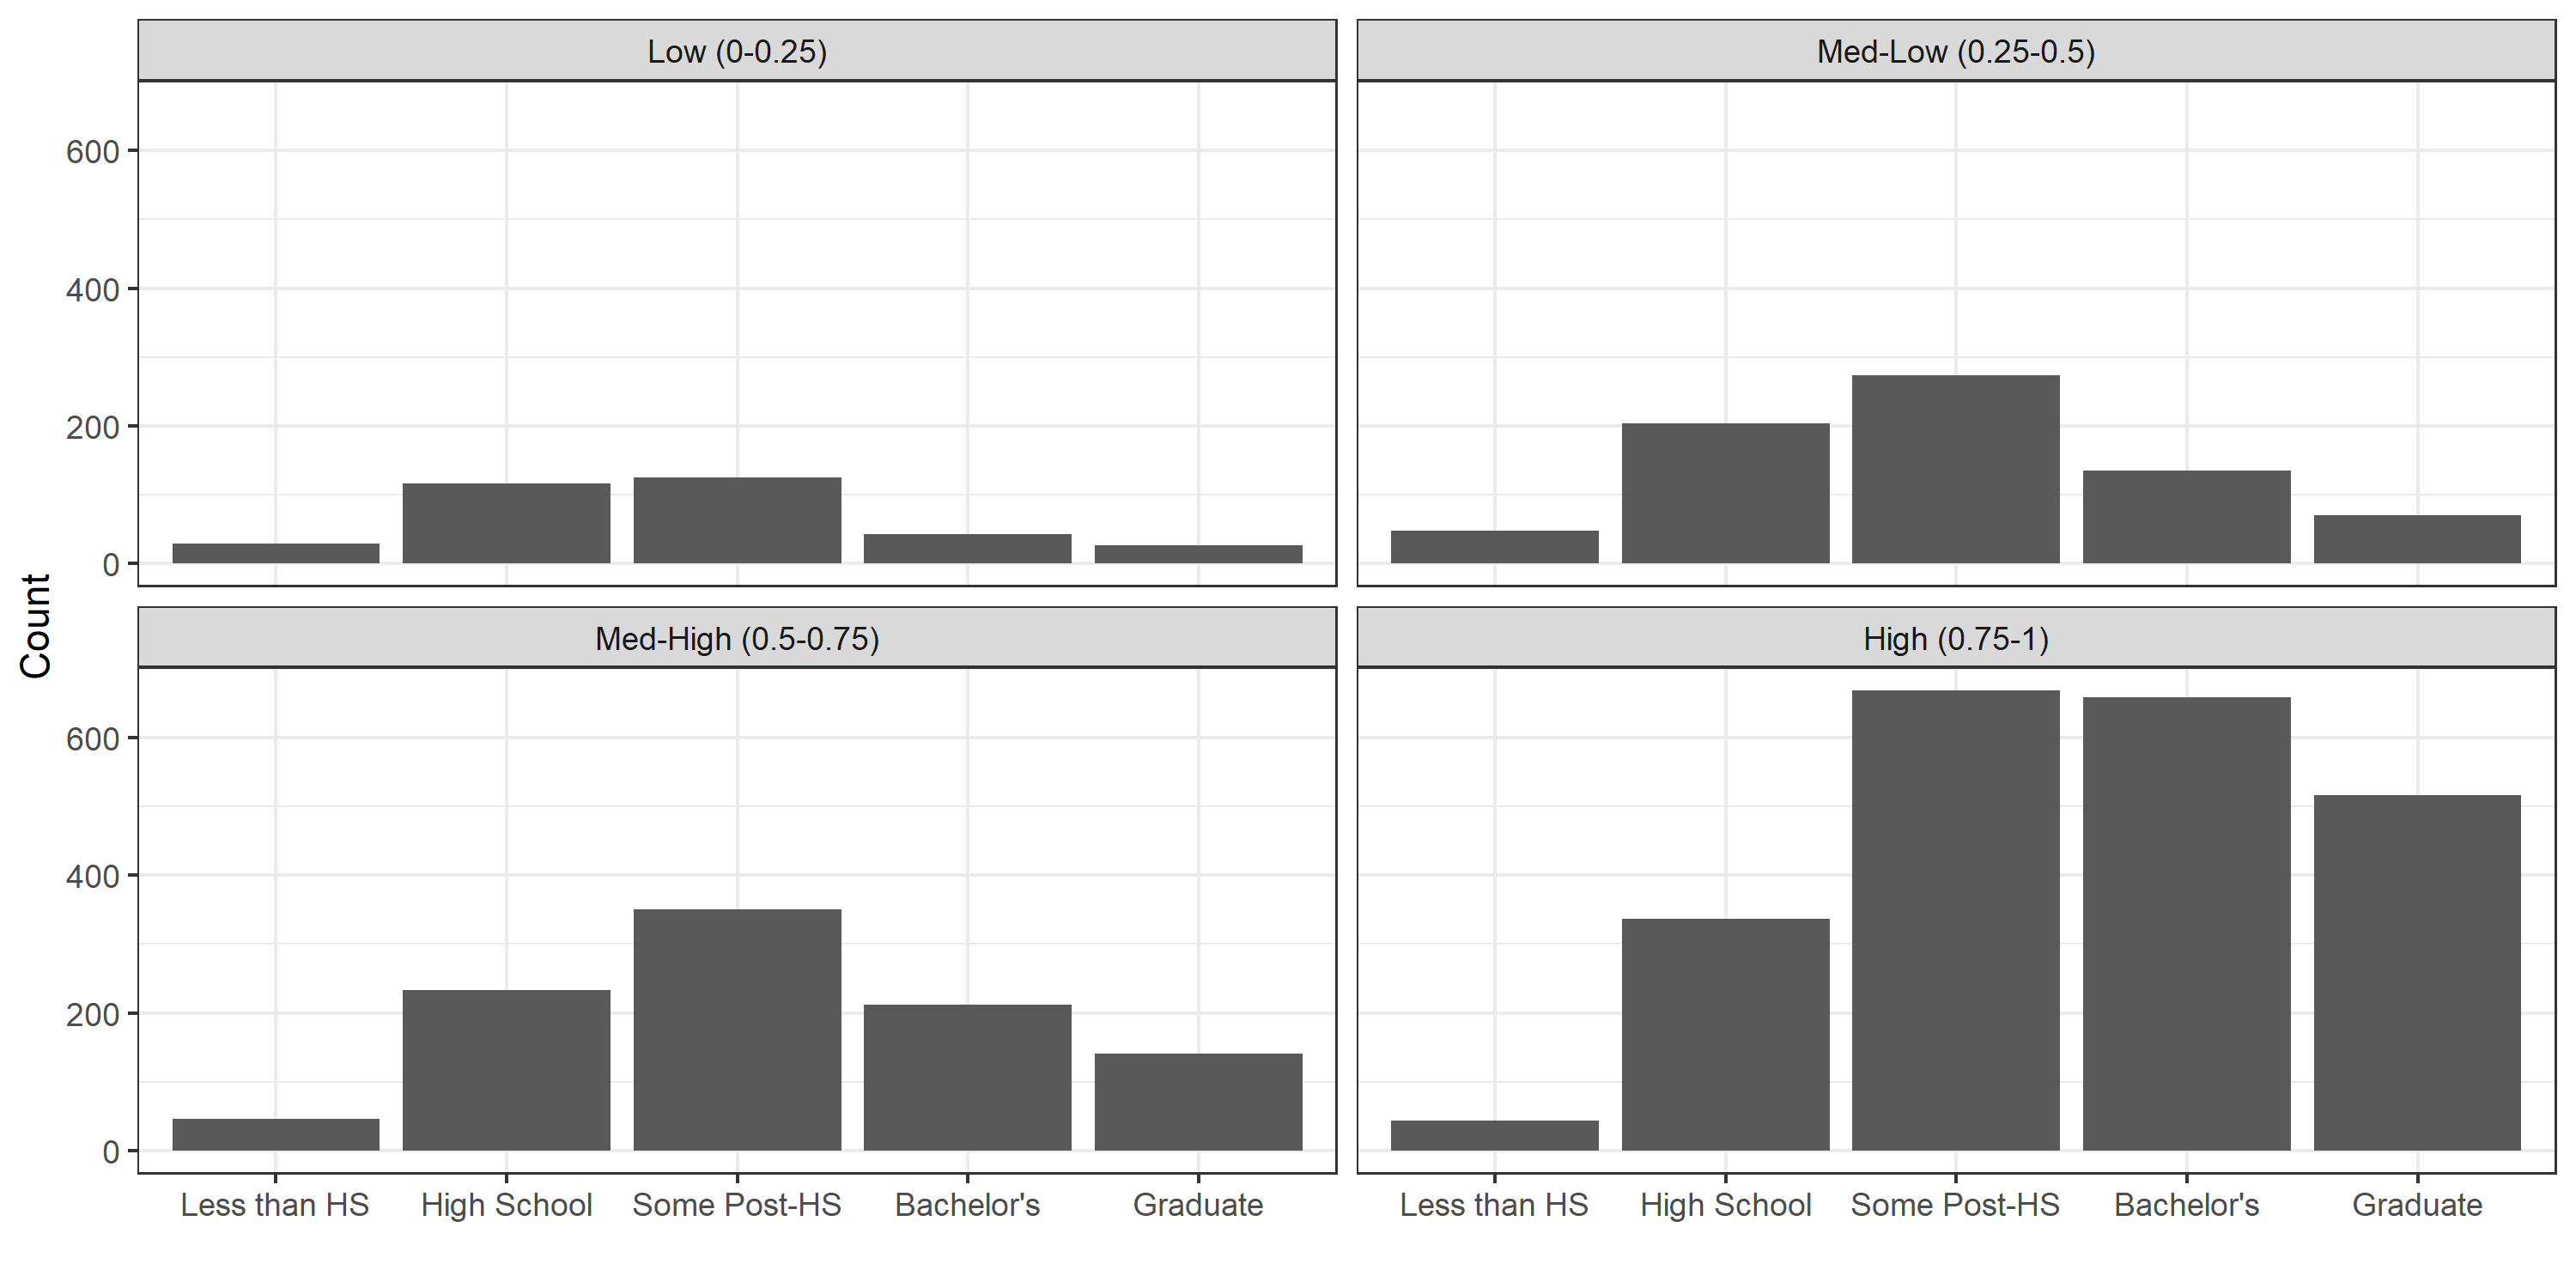
\includegraphics[scale=.5]{fig/soph-education.png}
	{\singlespacing
		\parbox{0.78\textwidth}{\scriptsize%\vspace{-0.25cm}
			Notes: Explain the figure here
	}}
	\caption{Distribution of Education Across Sophistication Quadrants}
	\label{educ}
\end{figure}


In addition to demographic controls, I employ a set of attitudinal items long believed to be relevant in explaining individual's symbolic racism scores \citep{kinder_divided_1997, sears_symbolic_1988}. These include measures of both partisanship and ideology, on the assumption that structuralist as opposed to individual explanations for social disadvantage are a hallmark of liberal Democratic thinking. Following \cite{feldman_structure_1988}, I include measures of individualist and egalitarian value orientations, measured outside the domain of race. I am unable to replicate the individualism scale constructed by \cite{henry_symbolic_2002}, which the original analysis uses, because the ANES has reduced its individualist orientation items to two. I use both items and adjust my scale accordingly.


\subsection{Descriptive Trends}

\begin{figure}[H]
	\centering
	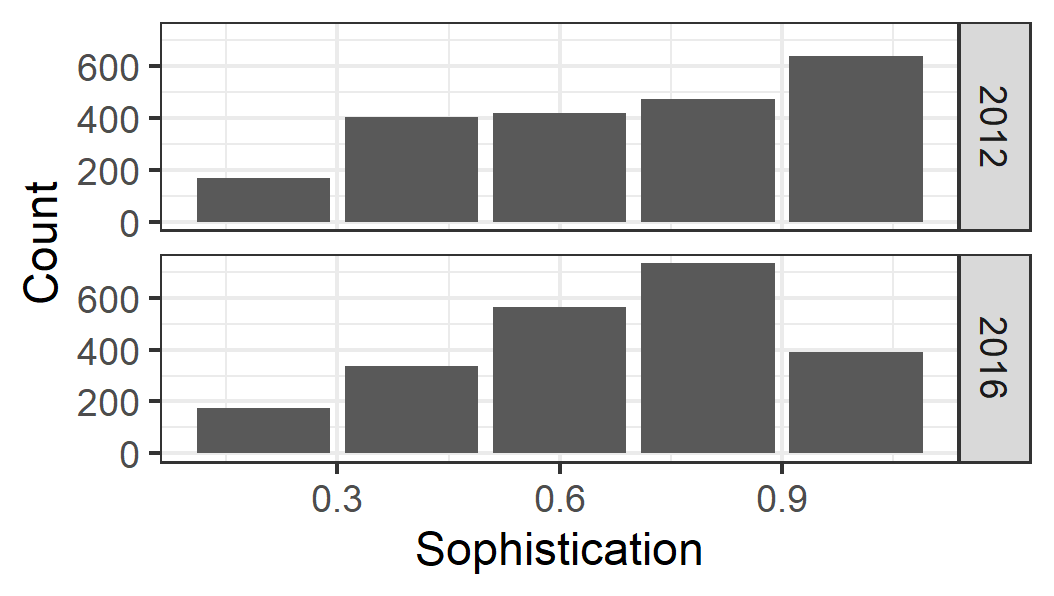
\includegraphics[scale=1]{fig/sophistication-desc.png}
	{\singlespacing
		\parbox{0.78\textwidth}{\scriptsize%\vspace{-0.25cm}
			Notes: Explain the figure here
	}}
	\caption{Distribution of Sophistication Across Years}
	\label{soph}
\end{figure}

Before estimating my models, I present descriptive trends within the data so that readers have a more nuanced understanding of the underlying shape and distributions of key variables. Figure \ref{soph} shows the distribution of political sophistication scores across the sample in 2012 and 2016. While both distributions are left skewed, there are plenty of low-sophisticates in the sample, indicating that we have appropriate variation in the independent variable to comment on the behavior of high and low sophisticates. In 2012, sophistication scores range from $0-1$ with a mean of $0.69$; in 2016, the range is $0-1$ and the mean is $0.66$.

\begin{figure}[H]
	\centering
	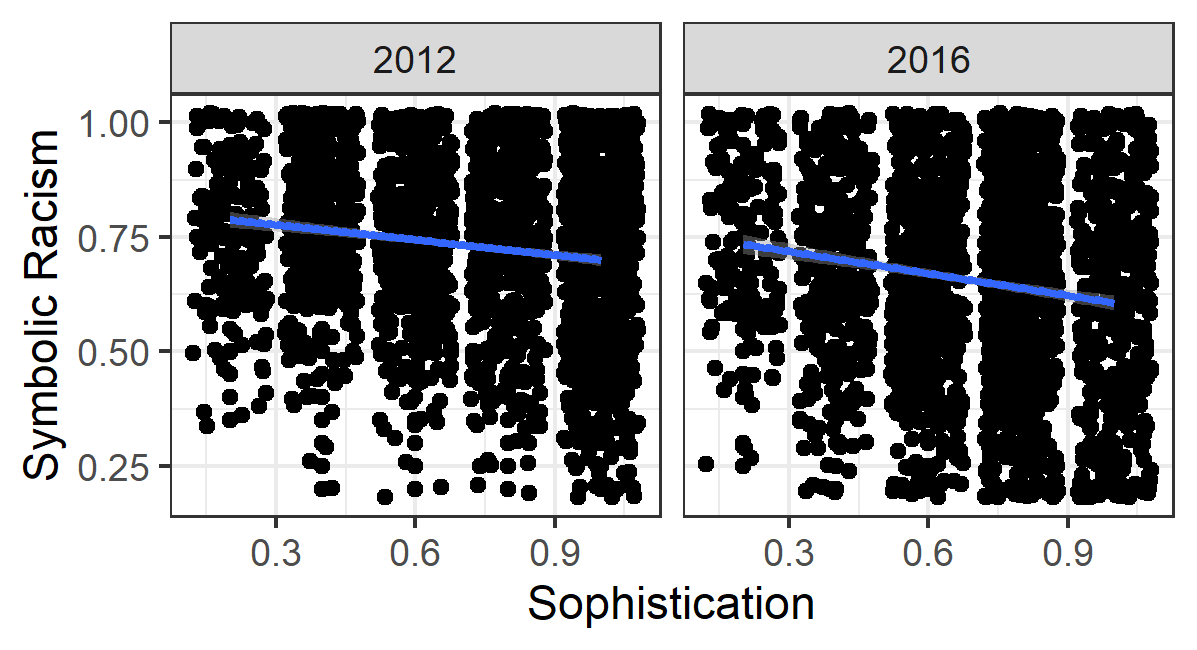
\includegraphics[scale=1]{fig/symbolic-racism-desc.png}
	{\singlespacing
		\parbox{0.78\textwidth}{\scriptsize%\vspace{-0.25cm}
			Notes: Explain the figure here
	}}
	\caption{Covariance in Symbolic Racism Score and Sophistication}
	\label{symbol-rac}
\end{figure}

Figure \ref{symbol-rac} plots respondents' symbolic racism scores against their political sophistication.  In 2012, symbolic racism scores range from $0.2-1$ with a mean of $0.73$; in 2016, the range is $0.2-1$ and the mean is $0.66$. The relationship between sophistication and symbolic racism is weakly negative. In general, as political sophistication increases, we observe a weak decrease in symbolic racism scores.

\begin{figure}[H]
	\centering
	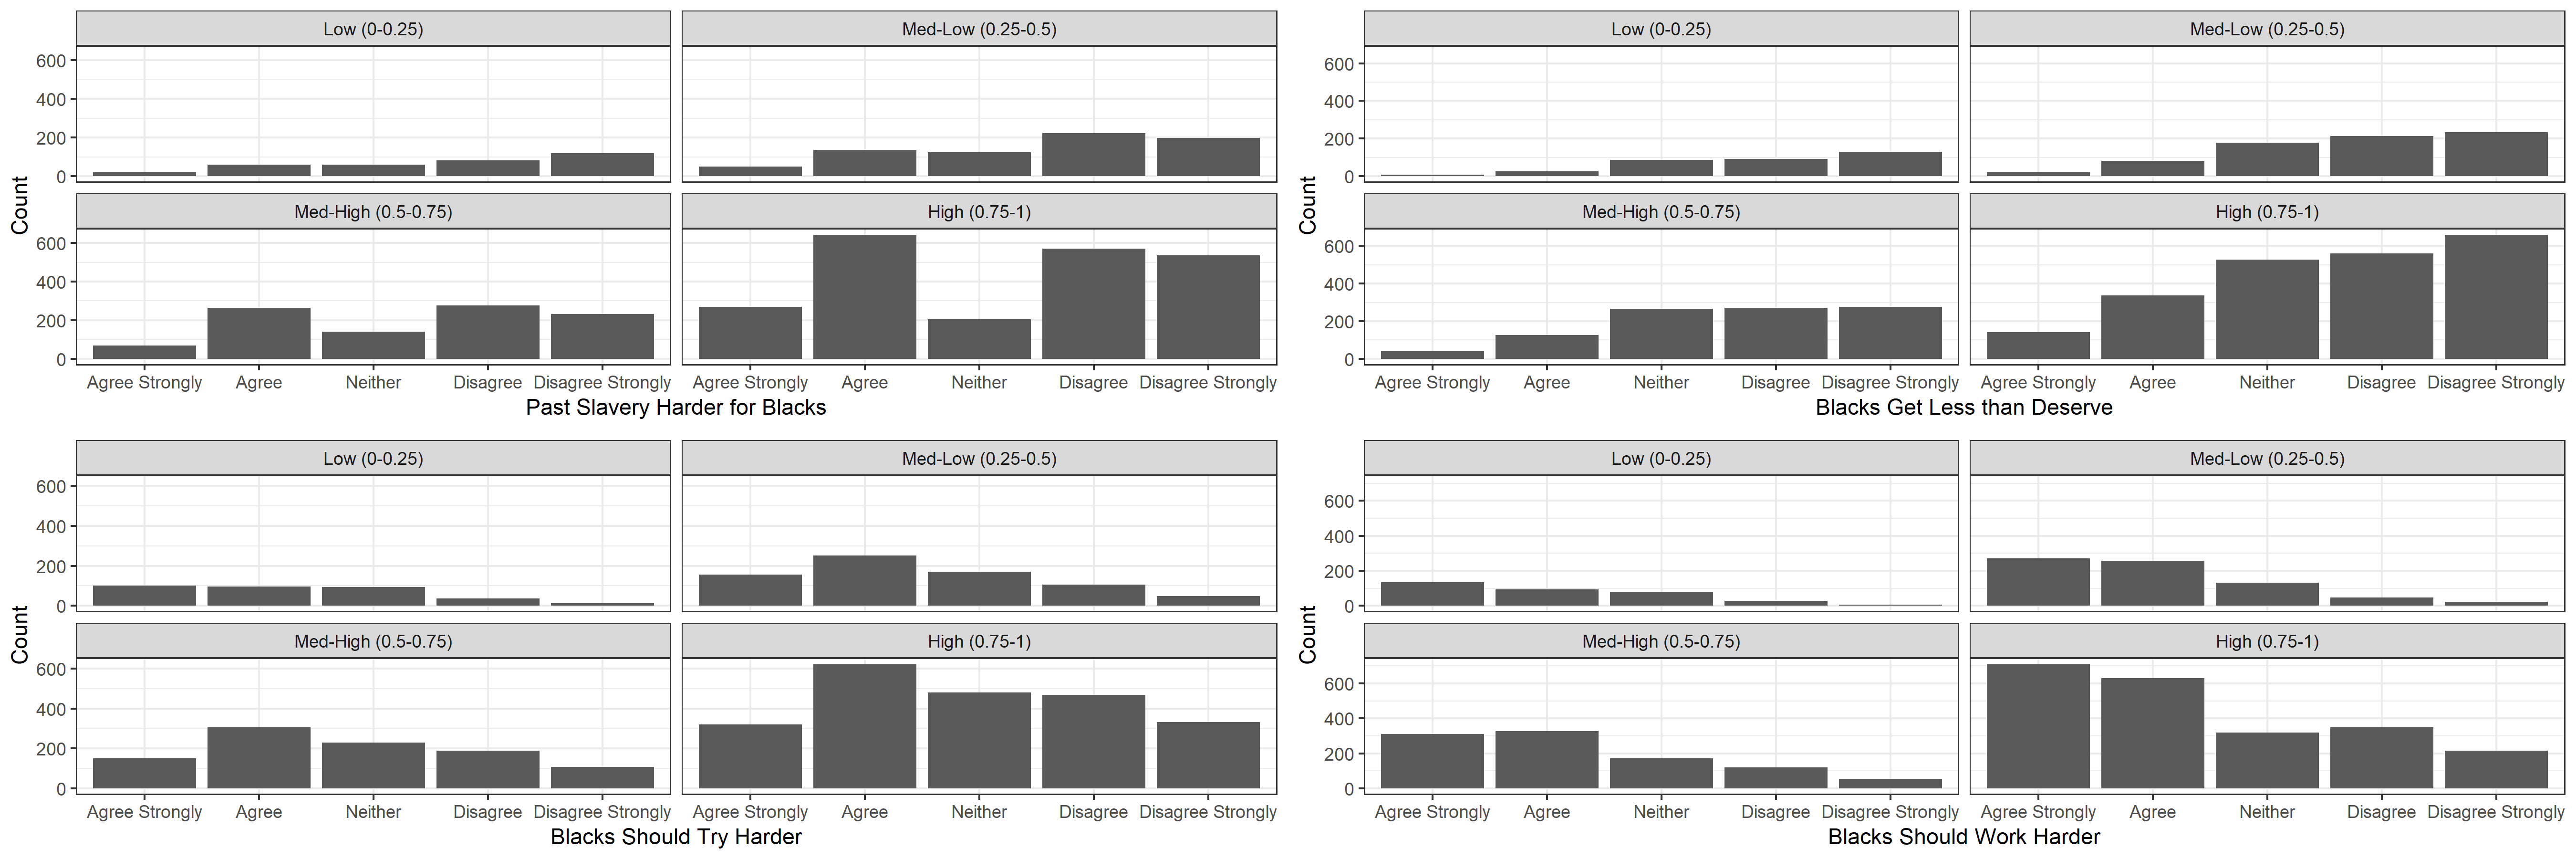
\includegraphics[scale=.4]{fig/response-by-soph.png}
	{\singlespacing
		\parbox{0.78\textwidth}{\scriptsize%\vspace{-0.25cm}
			Notes: Explain the figure here
	}}
	\caption{Symbolic Racism Item Responses by Sophistication}
	\label{response-soph}
\end{figure}

Recall that \cite{gomez_rethinking_2006} assert that non-racists who are simply politically unsophisticated may be incorrectly classified as racist by standard measures of symbolic racism using data from the 20th Century. I argue that political sophistication in the 21st Century is easier to obtain than in the 20th century. That is, as political information proliferates, it is easier for people to become passively informed about the state of the world. If this is the case, then we should expect to see a high proportion of respondents classified as politically sophisticated and less clear-cut distinctions between high and low sophisticates. Indeed, Figure \ref{response-soph} shows that far more respondents are in the upper sophistication quadrant than any other and appear, as a group, ambivalent regarding whether black poverty is a product of individual failings or structural hardship. These descriptive trends bolster my expectation that we should find no significant relationship between political sophistication and the likelihood of making a structuralist attribution.

\section{Empirical Results}
%corresponds to G&W06 Table 1
\begin{table}[!h] \centering 
	\caption{Model 1 (OLS)} 
	\label{ols} 
	\begin{tabular}{@{\extracolsep{5pt}}lD{.}{.}{-3} D{.}{.}{-3} } 
		\\[-1.8ex]\hline \\[-1.8ex] 
		\\[-1.8ex] & \multicolumn{2}{c}{Symbolic Racism} \\ 
		\\[-1.8ex] & \multicolumn{1}{c}{(1)} & \multicolumn{1}{c}{(2)}\\ 
		\hline \\[-1.8ex] 
		Political Sophistication & -0.078^{***} & -0.057^{***} \\ 
		& (0.012) & (0.016) \\ 
		Female & 0.001 & 0.006 \\ 
		& (0.006) & (0.006) \\ 
		Education & -0.031^{***} & -0.037^{***} \\ 
		& (0.003) & (0.004) \\ 
		Economic Individualism & 0.076^{***} & 0.087^{***} \\ 
		& (0.009) & (0.010) \\ 
		Egalitarianism & -0.373^{***} & -0.414^{***} \\ 
		& (0.023) & (0.025) \\ 
		South & 0.021^{***} & 0.036^{***} \\ 
		& (0.007) & (0.007) \\ 
		Democrat & -0.018^{**} & -0.082^{***} \\ 
		& (0.008) & (0.009) \\ 
		Church Attendance & 0.011^{*} & -0.024^{***} \\ 
		& (0.006) & (0.007) \\ 
		Ideology & 0.017^{***} & 0.0004^{***} \\ 
		& (0.003) & (0.0001) \\ 
		Black Feeling Therm. & -0.001^{***} & -0.002^{***} \\ 
		& (0.0002) & (0.0002) \\ 
		Age & -0.0002 & 0.001^{***} \\ 
		& (0.0002) & (0.0002) \\ 
		Income & 0.001^{**} & -0.0003 \\ 
		& (0.0004) & (0.001) \\ 
		Constant & 1.061^{***} & 1.185^{***} \\ 
		& (0.031) & (0.029) \\ 
		N & \multicolumn{1}{c}{2,126} & \multicolumn{1}{c}{2,247} \\ 
		R$^{2}$ & \multicolumn{1}{c}{0.441} & \multicolumn{1}{c}{0.459} \\ 
		Adjusted R$^{2}$ & \multicolumn{1}{c}{0.438} & \multicolumn{1}{c}{0.456} \\ 
		Residual Std. Error & \multicolumn{1}{c}{0.142 (df = 2113)} & \multicolumn{1}{c}{0.166 (df = 2234)} \\ 
		F Statistic & \multicolumn{1}{c}{139.141$^{***}$ (df = 12; 2113)} & \multicolumn{1}{c}{157.899$^{***}$ (df = 12; 2234)} \\ 
		\hline \\[-1.8ex] 
		\multicolumn{3}{l}{$^{*}$p $<$ .1; $^{**}$p $<$ .05; $^{***}$p $<$ .01} \\ 
	\end{tabular} 
\end{table} 

My analysis begins by examining the premise underlying the central claim of the argument: that political sophistication significantly decreases individuals’ scores on the symbolic racism scale, even controlling for all of the standard predictors. For both 2012 and 2016, I construct OLS models of symbolic racism among non-Hispanic whites. The dependent variable is an additive scale of the four items discussed above, normalized to range continuously between 0 and 1. Higher scores indicate a greater level of symbolic racism.

Table \ref{ols} shows the result of this regression. In both years, political sophistication has a significant, negative relationship with symbolic racism, corresponding to Gomez and Wilson's (2006) findings.

%corresponds to G&W06 Table 2
\begin{table}[!h] \centering 
	\caption{Individual Attributions 2012-2016} 
	\label{indiv} 
	\begin{adjustbox}{width=1\textwidth}
		\begin{tabular}{@{\extracolsep{5pt}}lD{.}{.}{-3} D{.}{.}{-3} D{.}{.}{-3} D{.}{.}{-3} } 
		\\[-1.8ex]\hline \\[-1.8ex] 
		\\[-1.8ex] & \multicolumn{1}{c}{Question 1 (2012)} & \multicolumn{1}{c}{Question 2 (2012)} & \multicolumn{1}{c}{Question 1 (2016)} & \multicolumn{1}{c}{Question 2 (2016)} \\ 
		\\[-1.8ex] & \multicolumn{1}{c}{(1)} & \multicolumn{1}{c}{(2)} & \multicolumn{1}{c}{(3)} & \multicolumn{1}{c}{(4)}\\ 
		\hline \\[-1.8ex] 
		Political Sophistication & -0.593^{***} & -0.319^{***} & -0.490^{***} & -0.348^{***} \\ 
		& (0.093) & (0.097) & (0.102) & (0.105) \\ 
		Female & -0.072 & 0.045 & -0.014 & 0.050 \\ 
		& (0.048) & (0.049) & (0.036) & (0.036) \\ 
		Education & -0.224^{***} & -0.212^{***} & -0.197^{***} & -0.224^{***} \\ 
		& (0.024) & (0.024) & (0.024) & (0.025) \\ 
		Economic Individualism & 0.339^{***} & 0.502^{***} & 0.316^{***} & 0.505^{***} \\ 
		& (0.071) & (0.073) & (0.062) & (0.064) \\ 
		Egalitarianism & -1.827^{***} & -2.246^{***} & -2.064^{***} & -1.889^{***} \\ 
		& (0.179) & (0.189) & (0.162) & (0.168) \\ 
		South & 0.167^{***} & 0.095^{*} & 0.182^{***} & 0.203^{***} \\ 
		& (0.050) & (0.052) & (0.048) & (0.050) \\ 
		Democrat & -0.076 & -0.165^{***} & -0.378^{***} & -0.498^{***} \\ 
		& (0.062) & (0.063) & (0.056) & (0.057) \\ 
		Church Attendance & 0.062 & -0.020 & -0.134^{***} & -0.109^{**} \\ 
		& (0.049) & (0.051) & (0.047) & (0.049) \\ 
		Ideology & 0.114^{***} & 0.098^{***} & 0.002^{***} & 0.002^{***} \\ 
		& (0.021) & (0.022) & (0.001) & (0.001) \\ 
		Black Feeling Therm. & -0.011^{***} & -0.009^{***} & -0.010^{***} & -0.011^{***} \\ 
		& (0.001) & (0.001) & (0.001) & (0.001) \\ 
		Age & 0.0002 & 0.003 & 0.006^{***} & 0.012^{***} \\ 
		& (0.001) & (0.002) & (0.001) & (0.001) \\ 
		Income & 0.005 & -0.002 & -0.003 & -0.005 \\ 
		& (0.003) & (0.003) & (0.003) & (0.003) \\ 
		N & \multicolumn{1}{c}{2,126} & \multicolumn{1}{c}{2,126} & \multicolumn{1}{c}{2,247} & \multicolumn{1}{c}{2,247} \\ 
		\hline \\[-1.8ex] 
		\multicolumn{5}{l}{$^{*}$p $<$ .1; $^{**}$p $<$ .05; $^{***}$p $<$ .01} \\ 
		\end{tabular} 
	\end{adjustbox}
\end{table} 


If the effect of political sophistication on symbolic racism is rooted in different causal attributions among sophisticates and non-sophisticates, we should see this pattern manifest in an analysis of the components of the systemic racism scale. Specifically, sophistication should dramatically decrease the likelihood that individuals will attribute racial disparities to character failings or lack of hard work, while
sharply increasing the tendency to ascribe causality to broad social factors. If, however, sophistication is no longer associated with a higher likelihood of making structuralist attributions, we should see no relationship between sophistication and ascribing causality to abstract, institutional factors. 

I begin with individualistic attributions. Table \ref{indiv} shows the results of an ordered probit model, which predicts the likelihood of answered Strongly Disagree, Disagree, Neutral, Agree, or Strongly Agree to Questions 1 and 2 from the individualistic attribution survey items on political sophistication and a battery of controls. Higher scores correspond to more agreement with the statements.

My findings echo \cite{gomez_rethinking_2006}: higher political sophistication is associated with a lower likelihood of attributing black poverty to individual-level characteristics and statistically significant at conventional levels. Warm feelings toward black Americans and Egalitarianism are also associated with lower agreement with individualistic attributions, while economic individualism and residing in the south is associated with higher agreement with individualistic attributions.

Table \ref{structure} shows the results of an ordered probit model, which predicts the likelihood of answered Strongly Disagree, Disagree, Neutral, Agree, or Strongly Agree to Question 1 and 2 from the structural attribution survey items on political sophistication and a battery of controls. Higher values in the dependent variables indicate disagreement and lower values indicate agreement. I find mixed support for my predictions. The coefficient estimates on Question 1 in 2012 and Question 2 in 2016 are insignificant at even the most liberal of conventional levels, in support of my predictions. The estimated coefficient on Question 1 in 2016 is significant only at the p$=0.1$ level. However, the estimated coefficient on political sophistication for Question 2 in 2012 is negative, in line with Gomez and Wilson's predictions, and significant at the p$=0.01$ level.

One way to interpret this result is that the information environment in the 21st Century was conducive to increasing the ability of low sophisticates to acknowledge structural explanations for black poverty, but political sophisticates were more capable of connecting these explanations to the institution of slavery. Indeed, if my argument about the spread of information about institutional racism over time holds, it follows that we should expect the relationship between sophistication and making structuralist attributions will decline over time, as structural attributions become more accessible to low-sophisticates. Thus, that we observe significant and negative coefficients in 2012, but insignificant (at conventional levels) coefficients in 2016 is in line with my broader theoretical argument.

%corresponds to G&W06 Table 3
\begin{table}[H] \centering 
	\caption{Structural Attributions 2012-2016} 
	\label{structure} 
	\begin{adjustbox}{width=1\textwidth}
		\begin{tabular}{@{\extracolsep{5pt}}lD{.}{.}{-3} D{.}{.}{-3} D{.}{.}{-3} D{.}{.}{-3} } 
			\\[-1.8ex]\hline \\[-1.8ex] 
			\\[-1.8ex] & \multicolumn{1}{c}{Question 1 (2012)} & \multicolumn{1}{c}{Question 2 (2012)} & \multicolumn{1}{c}{Question 1 (2016)} & \multicolumn{1}{c}{Question 2 (2016)} \\ 
			\\[-1.8ex] & \multicolumn{1}{c}{(1)} & \multicolumn{1}{c}{(2)} & \multicolumn{1}{c}{(3)} & \multicolumn{1}{c}{(4)}\\ 
			\hline \\[-1.8ex] 
			Political Sophistication & -0.131 & -0.436^{***} & -0.194^{*} & -0.092 \\ 
			& (0.095) & (0.095) & (0.103) & (0.103) \\ 
			Female & 0.034 & 0.037 & 0.010 & 0.065^{*} \\ 
			& (0.049) & (0.048) & (0.036) & (0.036) \\ 
			Education & -0.111^{***} & -0.150^{***} & -0.154^{***} & -0.158^{***} \\ 
			& (0.024) & (0.024) & (0.024) & (0.024) \\ 
			Economic Individualism & 0.350^{***} & 0.385^{***} & 0.435^{***} & 0.386^{***} \\ 
			& (0.072) & (0.072) & (0.063) & (0.063) \\ 
			Egalitarianism & -2.245^{***} & -2.412^{***} & -2.182^{***} & -2.112^{***} \\ 
			& (0.187) & (0.184) & (0.165) & (0.164) \\ 
			South & 0.165^{***} & 0.093^{*} & 0.201^{***} & 0.134^{***} \\ 
			& (0.052) & (0.051) & (0.049) & (0.049) \\ 
			Democrat & -0.062 & -0.064 & -0.362^{***} & -0.299^{***} \\ 
			& (0.063) & (0.063) & (0.056) & (0.057) \\ 
			Church Attendance & 0.116^{**} & 0.115^{**} & -0.116^{**} & -0.121^{**} \\ 
			& (0.050) & (0.050) & (0.048) & (0.048) \\ 
			Ideology & 0.097^{***} & 0.073^{***} & 0.001 & 0.003^{***} \\ 
			& (0.021) & (0.021) & (0.001) & (0.001) \\ 
			Black Feeling Therm. & -0.007^{***} & -0.004^{***} & -0.010^{***} & -0.008^{***} \\ 
			& (0.001) & (0.001) & (0.001) & (0.001) \\ 
			Age & -0.001 & -0.005^{***} & 0.004^{***} & 0.002 \\ 
			& (0.002) & (0.002) & (0.001) & (0.001) \\ 
			Income & 0.011^{***} & 0.007^{**} & 0.001 & 0.002 \\ 
			& (0.003) & (0.003) & (0.003) & (0.003) \\ 
			N & \multicolumn{1}{c}{2,126} & \multicolumn{1}{c}{2,126} & \multicolumn{1}{c}{2,247} & \multicolumn{1}{c}{2,247} \\ 
			\hline \\[-1.8ex] 
			\multicolumn{5}{l}{$^{*}$p $<$ .1; $^{**}$p $<$ .05; $^{***}$p $<$ .01} \\ 
				\end{tabular} 
	\end{adjustbox}
\end{table} 


\section{Diagnostics and Robustness}
This section presents a series of diagnostic and fit tests in order to better contextualize the results presented above.

\subsection{OLS Model}
To examine the appropriateness of the analysis presented in \ref{ols}, I first fit a normal probability plot. This assesses the normality of the distribution of the underlying data by plotting observed data quantiles against quantiles from a normal distribution. If the data are normally distributed, the points on the normal probability plot should coalesce around the 45-degree line. Indeed, \ref{qq} shows that the points coalesce along the 45-degree line, indicating normally distributed data. While normally distributed data is not necessary for OLS to produce non-biased estimates, this plot gives us a better sense of the underlying distribution of the data we're using in our model.

\begin{figure}[h!]
	\centering
	\subfloat[\centering 2012]{{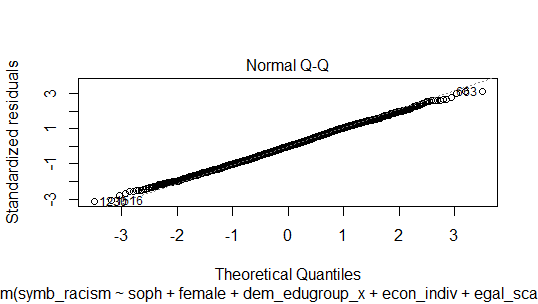
\includegraphics[width=5cm]{fig/qq-12.png} }}%
	\qquad
	\subfloat[\centering 2016]{{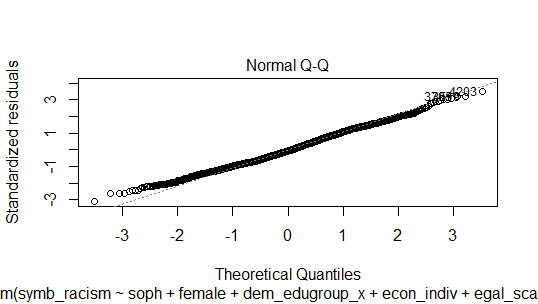
\includegraphics[width=5cm]{fig/qq-16.png} }}%
	\caption{Normal Q-Q Plots for 2012-2016 OLS Models}%
	\label{qq}%
\end{figure}

To assess the OLS models for linearity and heteroskedasticity, as well as get a sense for whether there are outliers, I plot the residuals over the fitted values for both 2012 and 2016 models. If the data meet homoskedasticity assumptions, we should see the points ``bounce" randomly above and below the 0 line. Instead, there is a clear trend of higher residuals for lower fitted values and lower residuals for higher fitted values. Indeed, Bruesch-Pagan testing confirms that we can reject the null hypothesis of homoskedasticity (p = $0.00$ for both years).


\begin{figure}%
	\centering
	\subfloat[\centering 2012]{{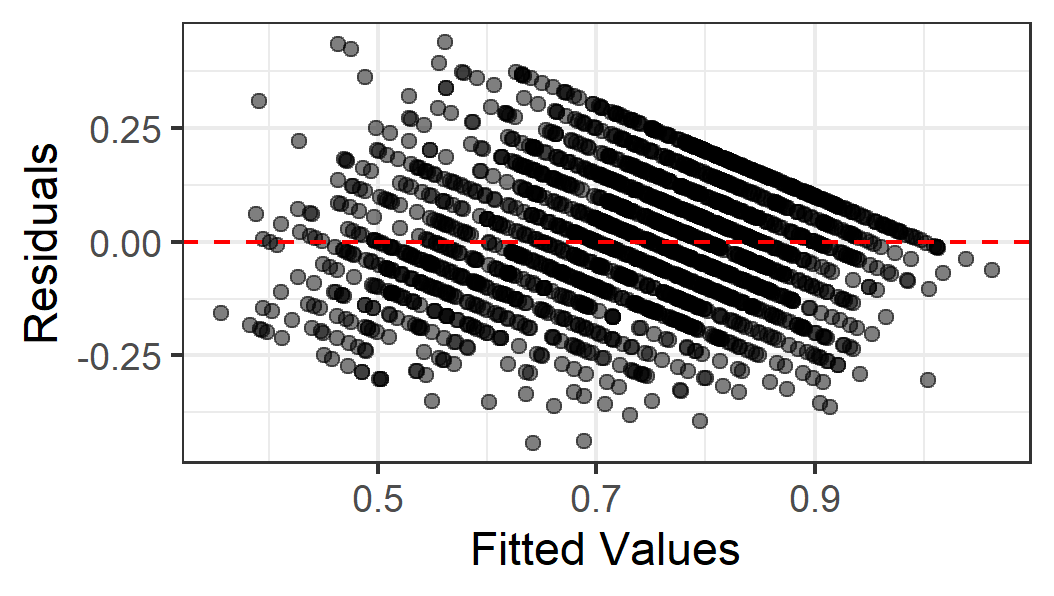
\includegraphics[width=5cm]{fig/resid-fitted-12.png} }}%
	\qquad
	\subfloat[\centering 2016]{{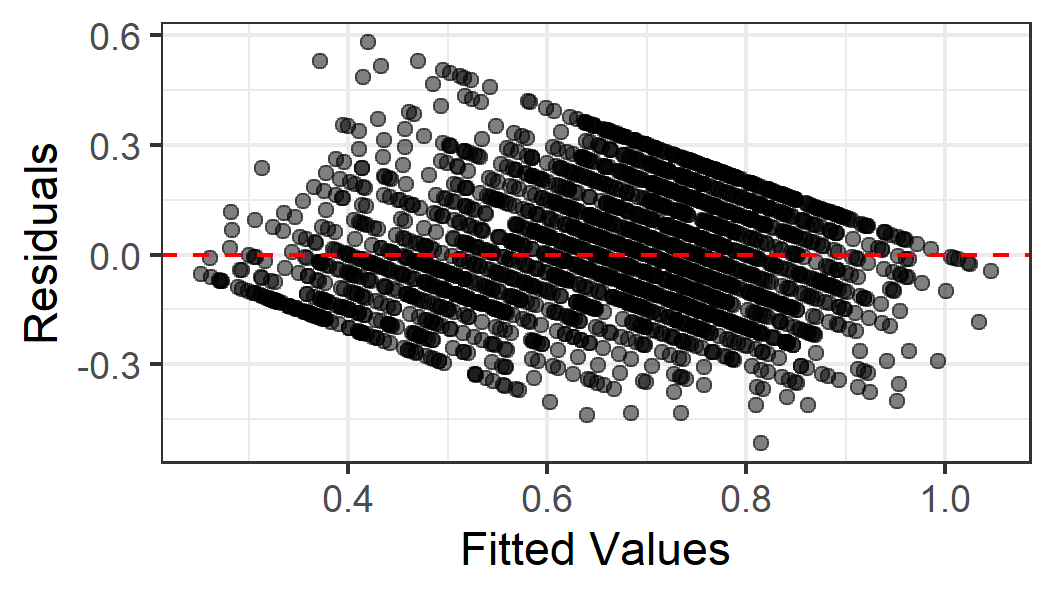
\includegraphics[width=5cm]{fig/resid-fitted-16.png} }}%
	\caption{Residuals vs Fitted Values Plots for 2012-2016 OLS Models}%
	\label{resid}%
\end{figure}

Given this, the model would be more appropriately estimated with heteroskedastic robust standard errors. Table \ref{rob} plots the original analysis from Table \ref{ols} in Columns 1 and 3 and the same models estimated with heteroskedastic robust standard errors in Columns 2 and 4. Substantively, the results do not change by much, nor does the  statistical significance.

\begin{table}[!htbp] 
	\centering 
	\caption{OLS with Normal vs. Robust SEs} 
	\label{rob} 
		\begin{adjustbox}{width=1\textwidth}
	\begin{tabular}{@{\extracolsep{5pt}}lD{.}{.}{-3} D{.}{.}{-3} D{.}{.}{-3} D{.}{.}{-3} } 
		\\[-1.8ex]\hline \\[-1.8ex] 
		\\[-1.8ex] & \multicolumn{4}{c}{Symbolic Racism} \\ 
		\\[-1.8ex] & \multicolumn{1}{c}{OLS} & \multicolumn{1}{c}{Heteroskedastic Robust SEs} & \multicolumn{1}{c}{OLS} & \multicolumn{1}{c}{Heteroskedastic Robust SEs} \\ 
		& \multicolumn{1}{c}{} & \multicolumn{1}{c}{} & \multicolumn{1}{c}{} & \multicolumn{1}{c}{} \\ 
		\\[-1.8ex] & \multicolumn{1}{c}{2012} & \multicolumn{1}{c}{2012} & \multicolumn{1}{c}{2016} & \multicolumn{1}{c}{2016}\\ 
		\hline \\[-1.8ex] 
		Political Sophistication & -0.078^{***} & -0.078^{***} & -0.057^{***} & -0.061^{***} \\ 
		& (0.012) & (0.013) & (0.016) & (0.017) \\ 
		Female & 0.001 & -0.0001 & 0.006 & 0.006 \\ 
		& (0.006) & (0.007) & (0.006) & (0.006) \\ 
		Education & -0.031^{***} & -0.031^{***} & -0.037^{***} & -0.038^{***} \\ 
		& (0.003) & (0.003) & (0.004) & (0.004) \\ 
		Economic Individualism & 0.076^{***} & 0.077^{***} & 0.087^{***} & 0.090^{***} \\ 
		& (0.009) & (0.010) & (0.010) & (0.010) \\ 
		Egalitarianism & -0.373^{***} & -0.384^{***} & -0.414^{***} & -0.438^{***} \\ 
		& (0.023) & (0.026) & (0.025) & (0.028) \\ 
		South & 0.021^{***} & 0.024^{***} & 0.036^{***} & 0.040^{***} \\ 
		& (0.007) & (0.007) & (0.007) & (0.008) \\ 
		Democrat & -0.018^{**} & -0.017^{*} & -0.082^{***} & -0.082^{***} \\ 
		& (0.008) & (0.009) & (0.009) & (0.010) \\ 
		Church Attendance & 0.011^{*} & 0.010 & -0.024^{***} & -0.025^{***} \\ 
		& (0.006) & (0.007) & (0.007) & (0.008) \\ 
		Ideology & 0.017^{***} & 0.018^{***} & 0.0004^{***} & 0.0004^{***} \\ 
		& (0.003) & (0.003) & (0.0001) & (0.0001) \\ 
		Black Feeling Therm. & -0.001^{***} & -0.001^{***} & -0.002^{***} & -0.002^{***} \\ 
		& (0.0002) & (0.0002) & (0.0002) & (0.0002) \\ 
		Age & -0.0002 & -0.0002 & 0.001^{***} & 0.001^{***} \\ 
		& (0.0002) & (0.0002) & (0.0002) & (0.0002) \\ 
		Income & 0.001^{**} & 0.001^{**} & -0.0003 & -0.0002 \\ 
		& (0.0004) & (0.0004) & (0.001) & (0.001) \\ 
		Constant & 1.061^{***} & 1.066^{***} & 1.185^{***} & 1.203^{***} \\ 
		& (0.031) & (0.034) & (0.029) & (0.030) \\ 
		N & \multicolumn{1}{c}{2,126} & \multicolumn{1}{c}{2,126} & \multicolumn{1}{c}{2,247} & \multicolumn{1}{c}{2,247} \\ 
		R$^{2}$ & \multicolumn{1}{c}{0.441} & \multicolumn{1}{c}{0.451} & \multicolumn{1}{c}{0.459} & \multicolumn{1}{c}{0.475} \\ 
		Adjusted R$^{2}$ & \multicolumn{1}{c}{0.438} & \multicolumn{1}{c}{0.448} & \multicolumn{1}{c}{0.456} & \multicolumn{1}{c}{0.472} \\ 
		Residual Std. Error & \multicolumn{1}{c}{0.142 (df = 2113)} & \multicolumn{1}{c}{0.144 (df = 2113)} & \multicolumn{1}{c}{0.166 (df = 2234)} & \multicolumn{1}{c}{0.170 (df = 2234)} \\ 
		F Statistic & \multicolumn{1}{c}{139.141$^{***}$ (df = 12; 2113)} &  & \multicolumn{1}{c}{157.899$^{***}$ (df = 12; 2234)} &  \\ 
		\hline \\[-1.8ex] 
		\multicolumn{5}{l}{$^{*}$p $<$ .1; $^{**}$p $<$ .05; $^{***}$p $<$ .01} \\ 
	\end{tabular} 
\end{adjustbox}
\end{table} 

\subsection{Ordered Probit Models}
I estimate surrogate residuals to run comparable diagnostics on my ordered probit models \citep{liu_residuals_2018}. Figure \ref{fitted-resid-12} shows the residuals over fitted values plots for each of the 2012 symbolic racism items, corresponding to Columns 1 and 2 in Table \ref{indiv} and Columns 1 and 2 in Table \ref{structure}. The surrogate residuals ``bounce" randomly around the zero line and do not demonstrate pronounced trends, suggesting that heteroskedasticity is not a concern for these models.

\begin{figure}[h!]
		\centering
	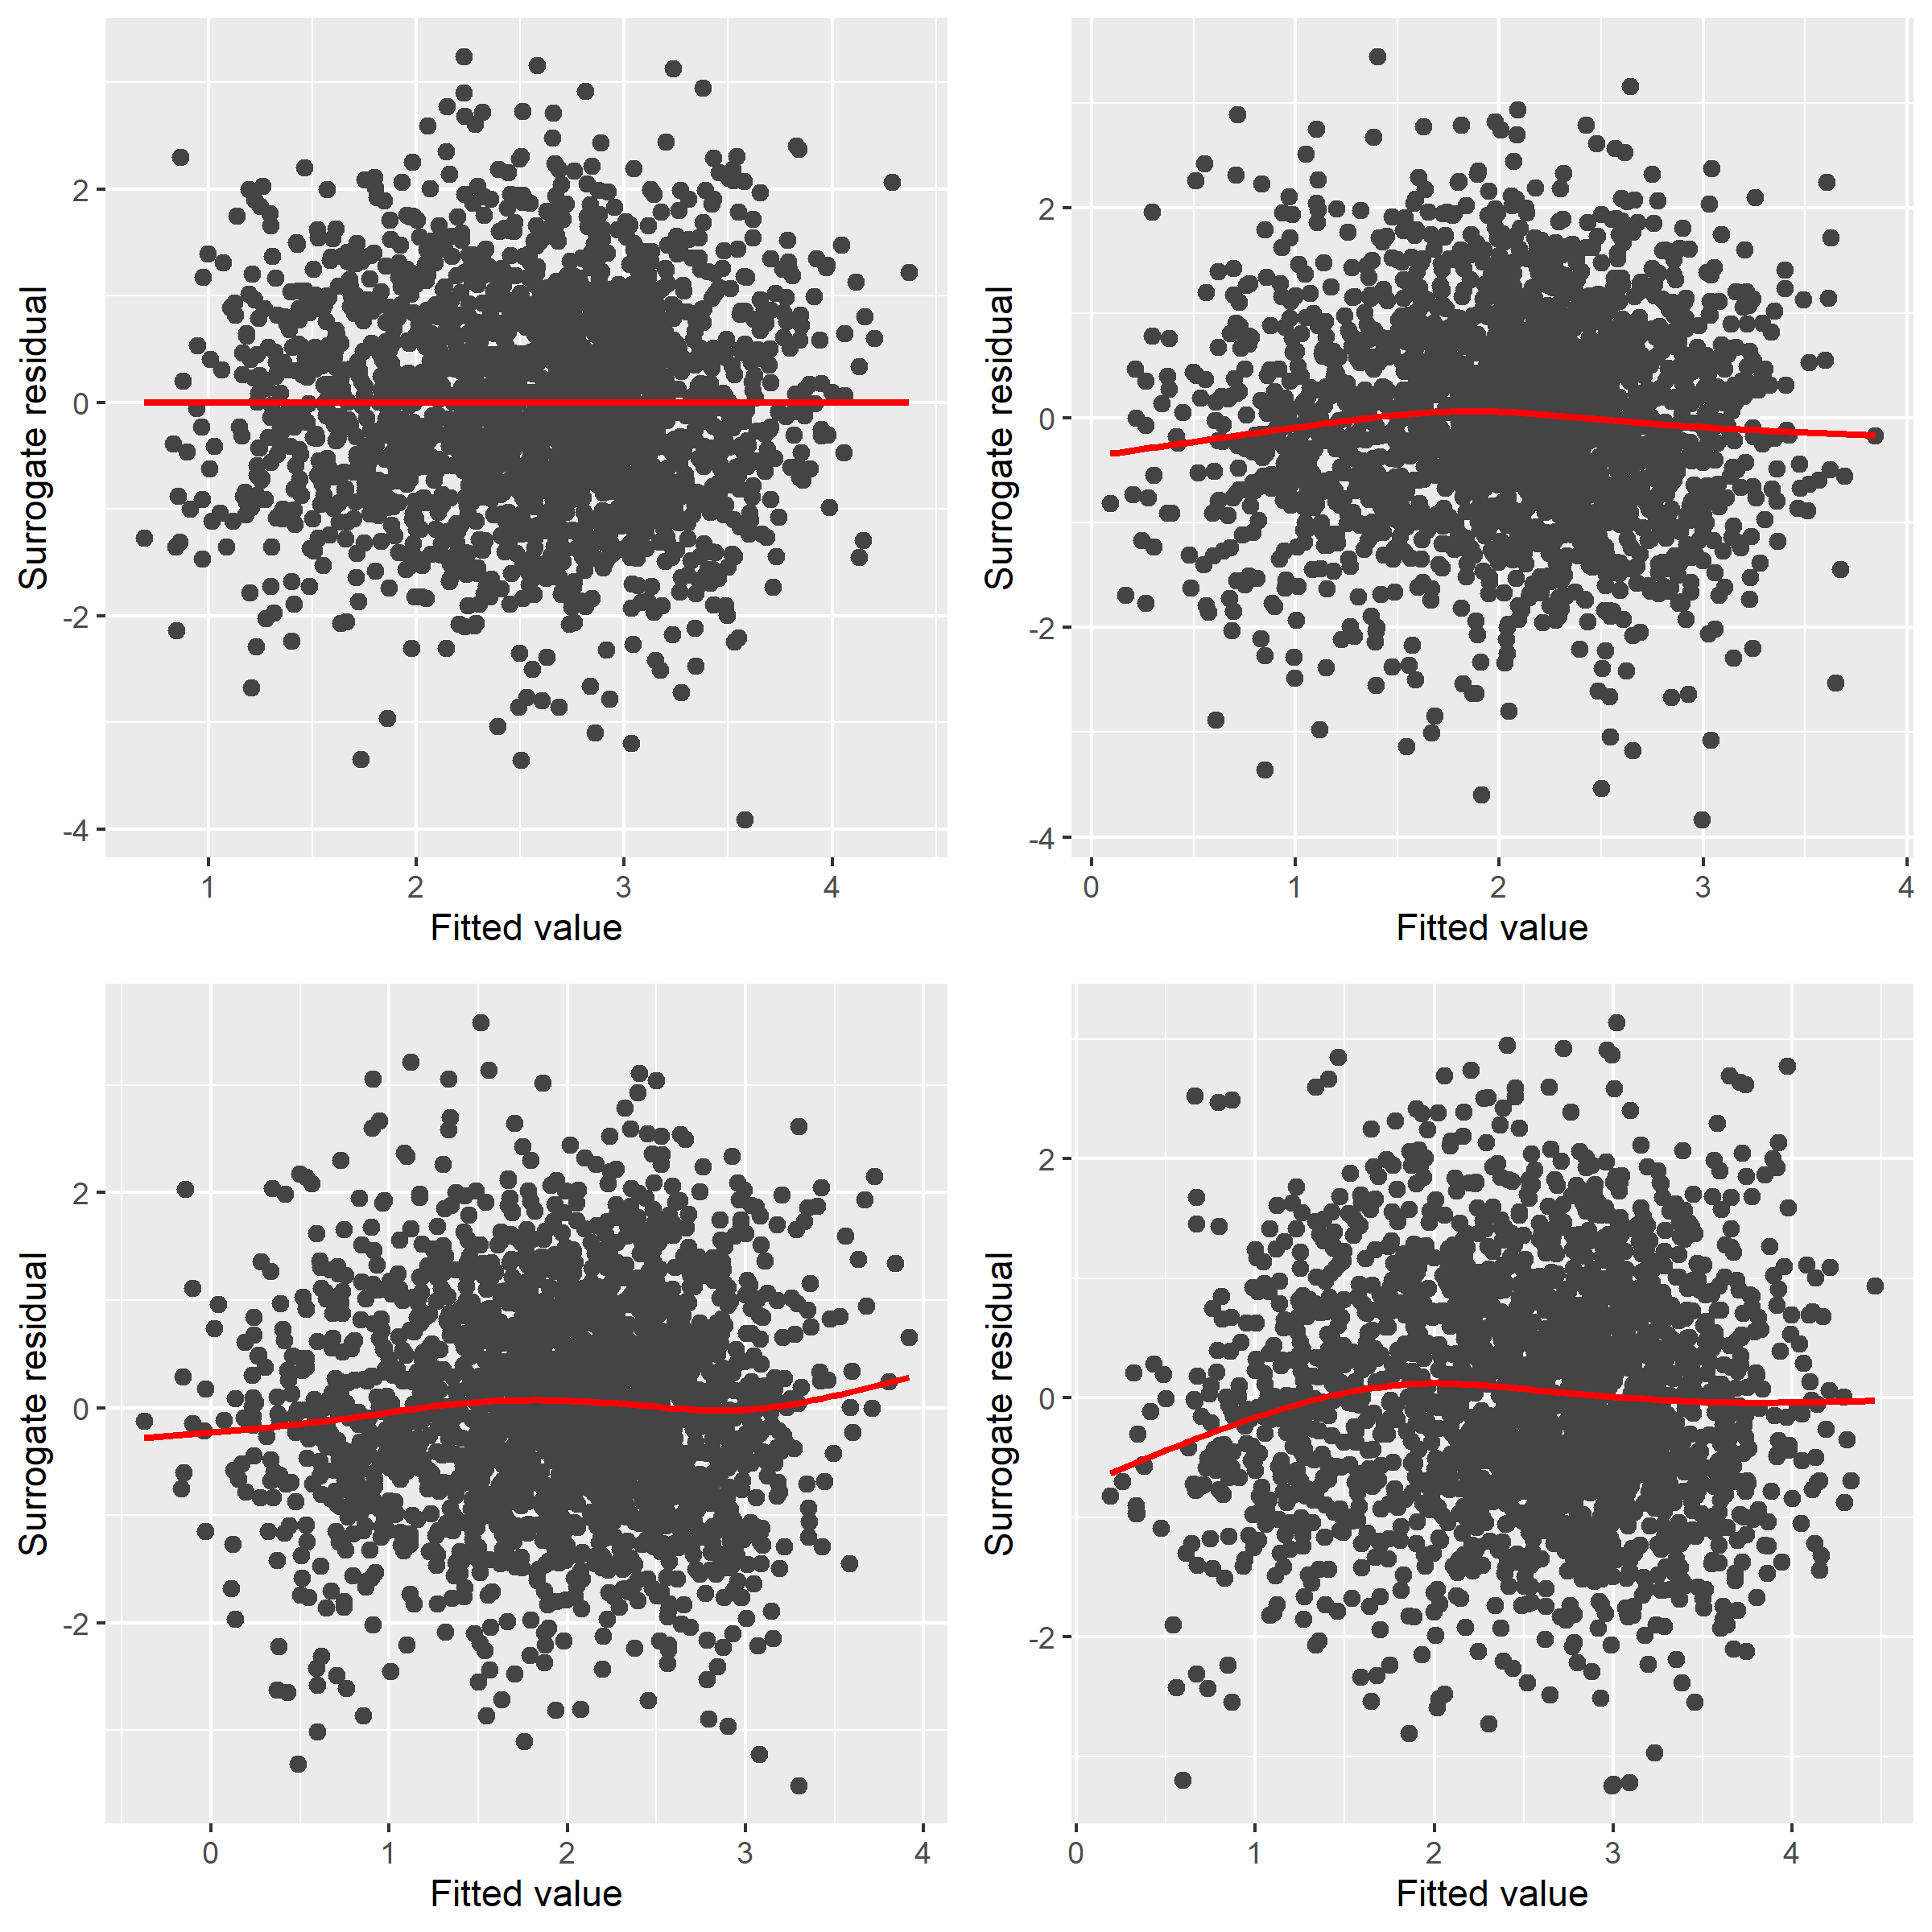
\includegraphics[scale=.55]{fig/fitted_residuals_12.png}
	%{\singlespacing
	%	\parbox{0.78\textwidth}{\scriptsize%\vspace{-0.25cm}
	%		Notes: Explain the figure here
	%}}
	\caption{Fitted Values over Residuals Plot for 2012 Symbolic Racism Items}
	\label{fitted-resid-12}
\end{figure}

Likewise, Figure \ref{fitted-resid-16} shows the same residuals over fitted values plot for Columns 3 and 4 in Table \ref{indiv} and Columns 3 and 4 in Table \ref{structure}. The surrogate residuals ``bounce" randomly around the zero line and do not demonstrate pronounced trends, suggesting that heteroskedasticity is not a concern for these models.

\begin{figure}[h!]
	\centering
	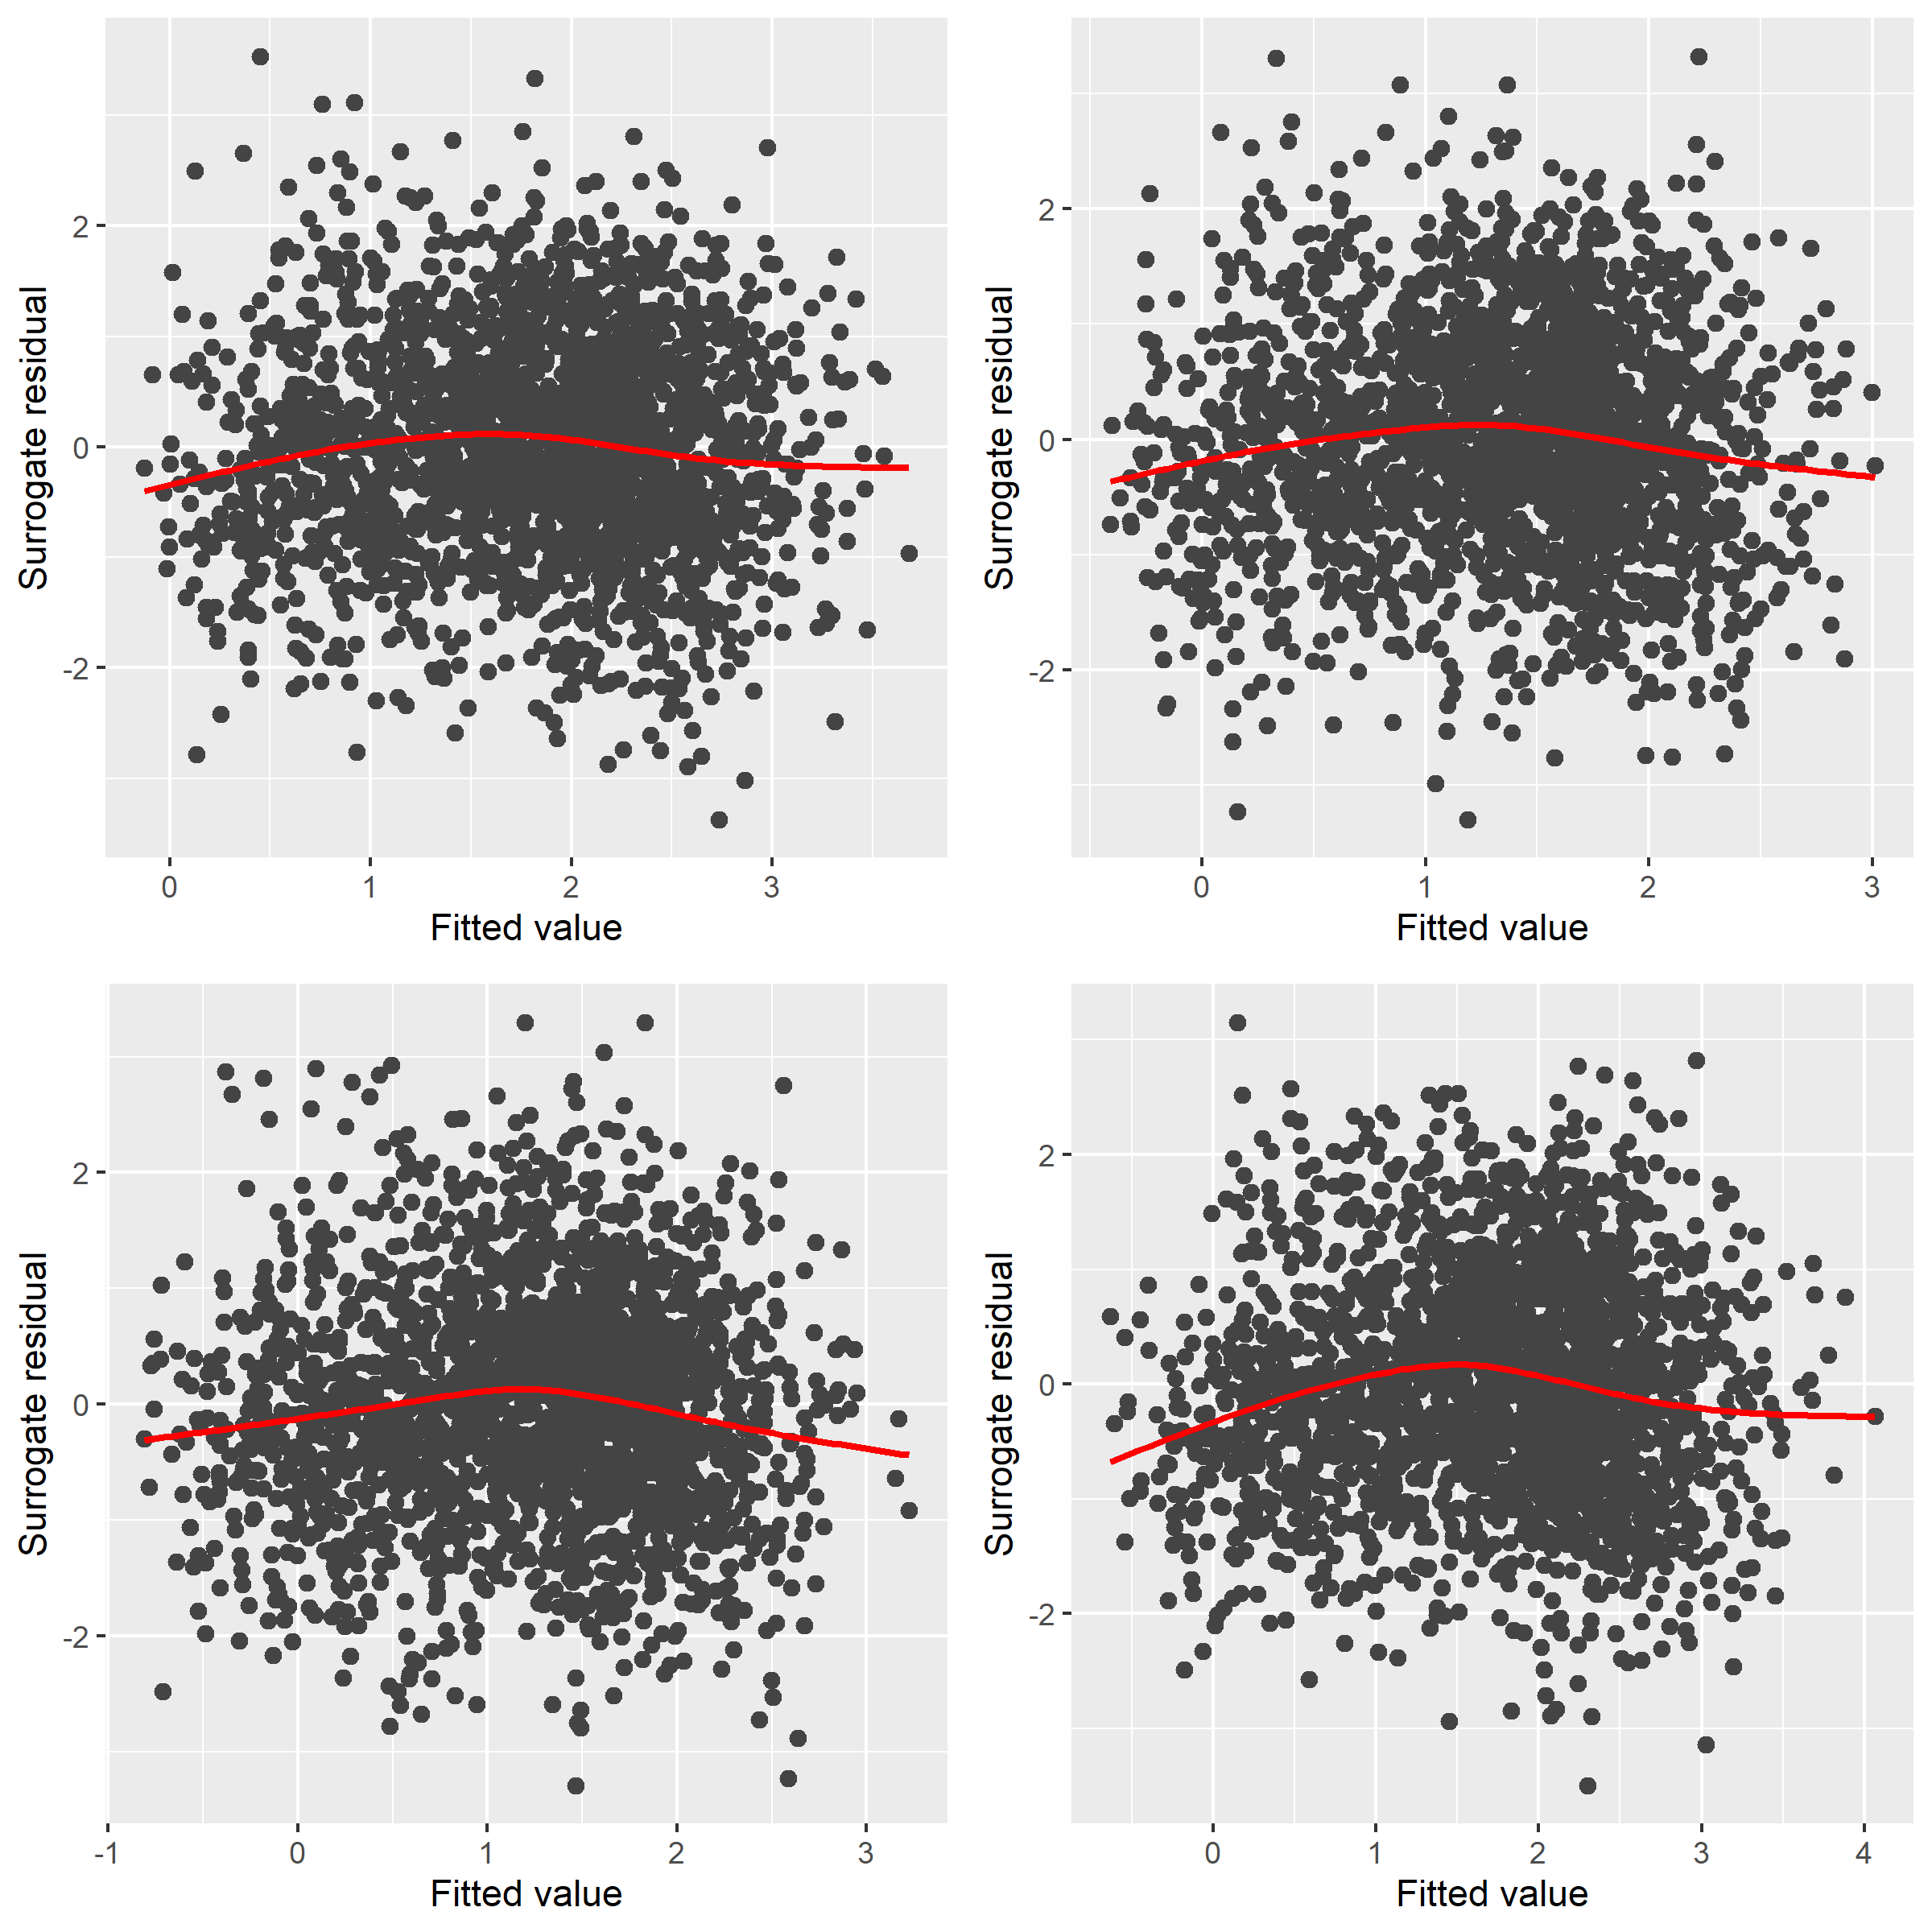
\includegraphics[scale=.55]{fig/fitted_residuals_16.png}
	%{\singlespacing
	%	\parbox{0.78\textwidth}{\scriptsize%\vspace{-0.25cm}
	%		Notes: Explain the figure here
	%}}
	\caption{Fitted Values over Residuals Plot for 2016 Symbolic Racism Items}
	\label{fitted-resid-16}
\end{figure}

To examine whether the data are normally distributed, I estimate normal probability plots for each of the ordered probit models in Table \ref{indiv} and Table \ref{structure} by plotting the observed quantiles in the data against normal theoretical quantiles.  If the two distributions are similar, observations should line up on the 45-degree line ($x=y$). As we can see from Figure \ref{qq-2}, the observations line up on the 45-degree line, indicating that the data are normally distributed. 

\begin{figure}[H]
	\centering
	\subfloat[\centering 2012]{{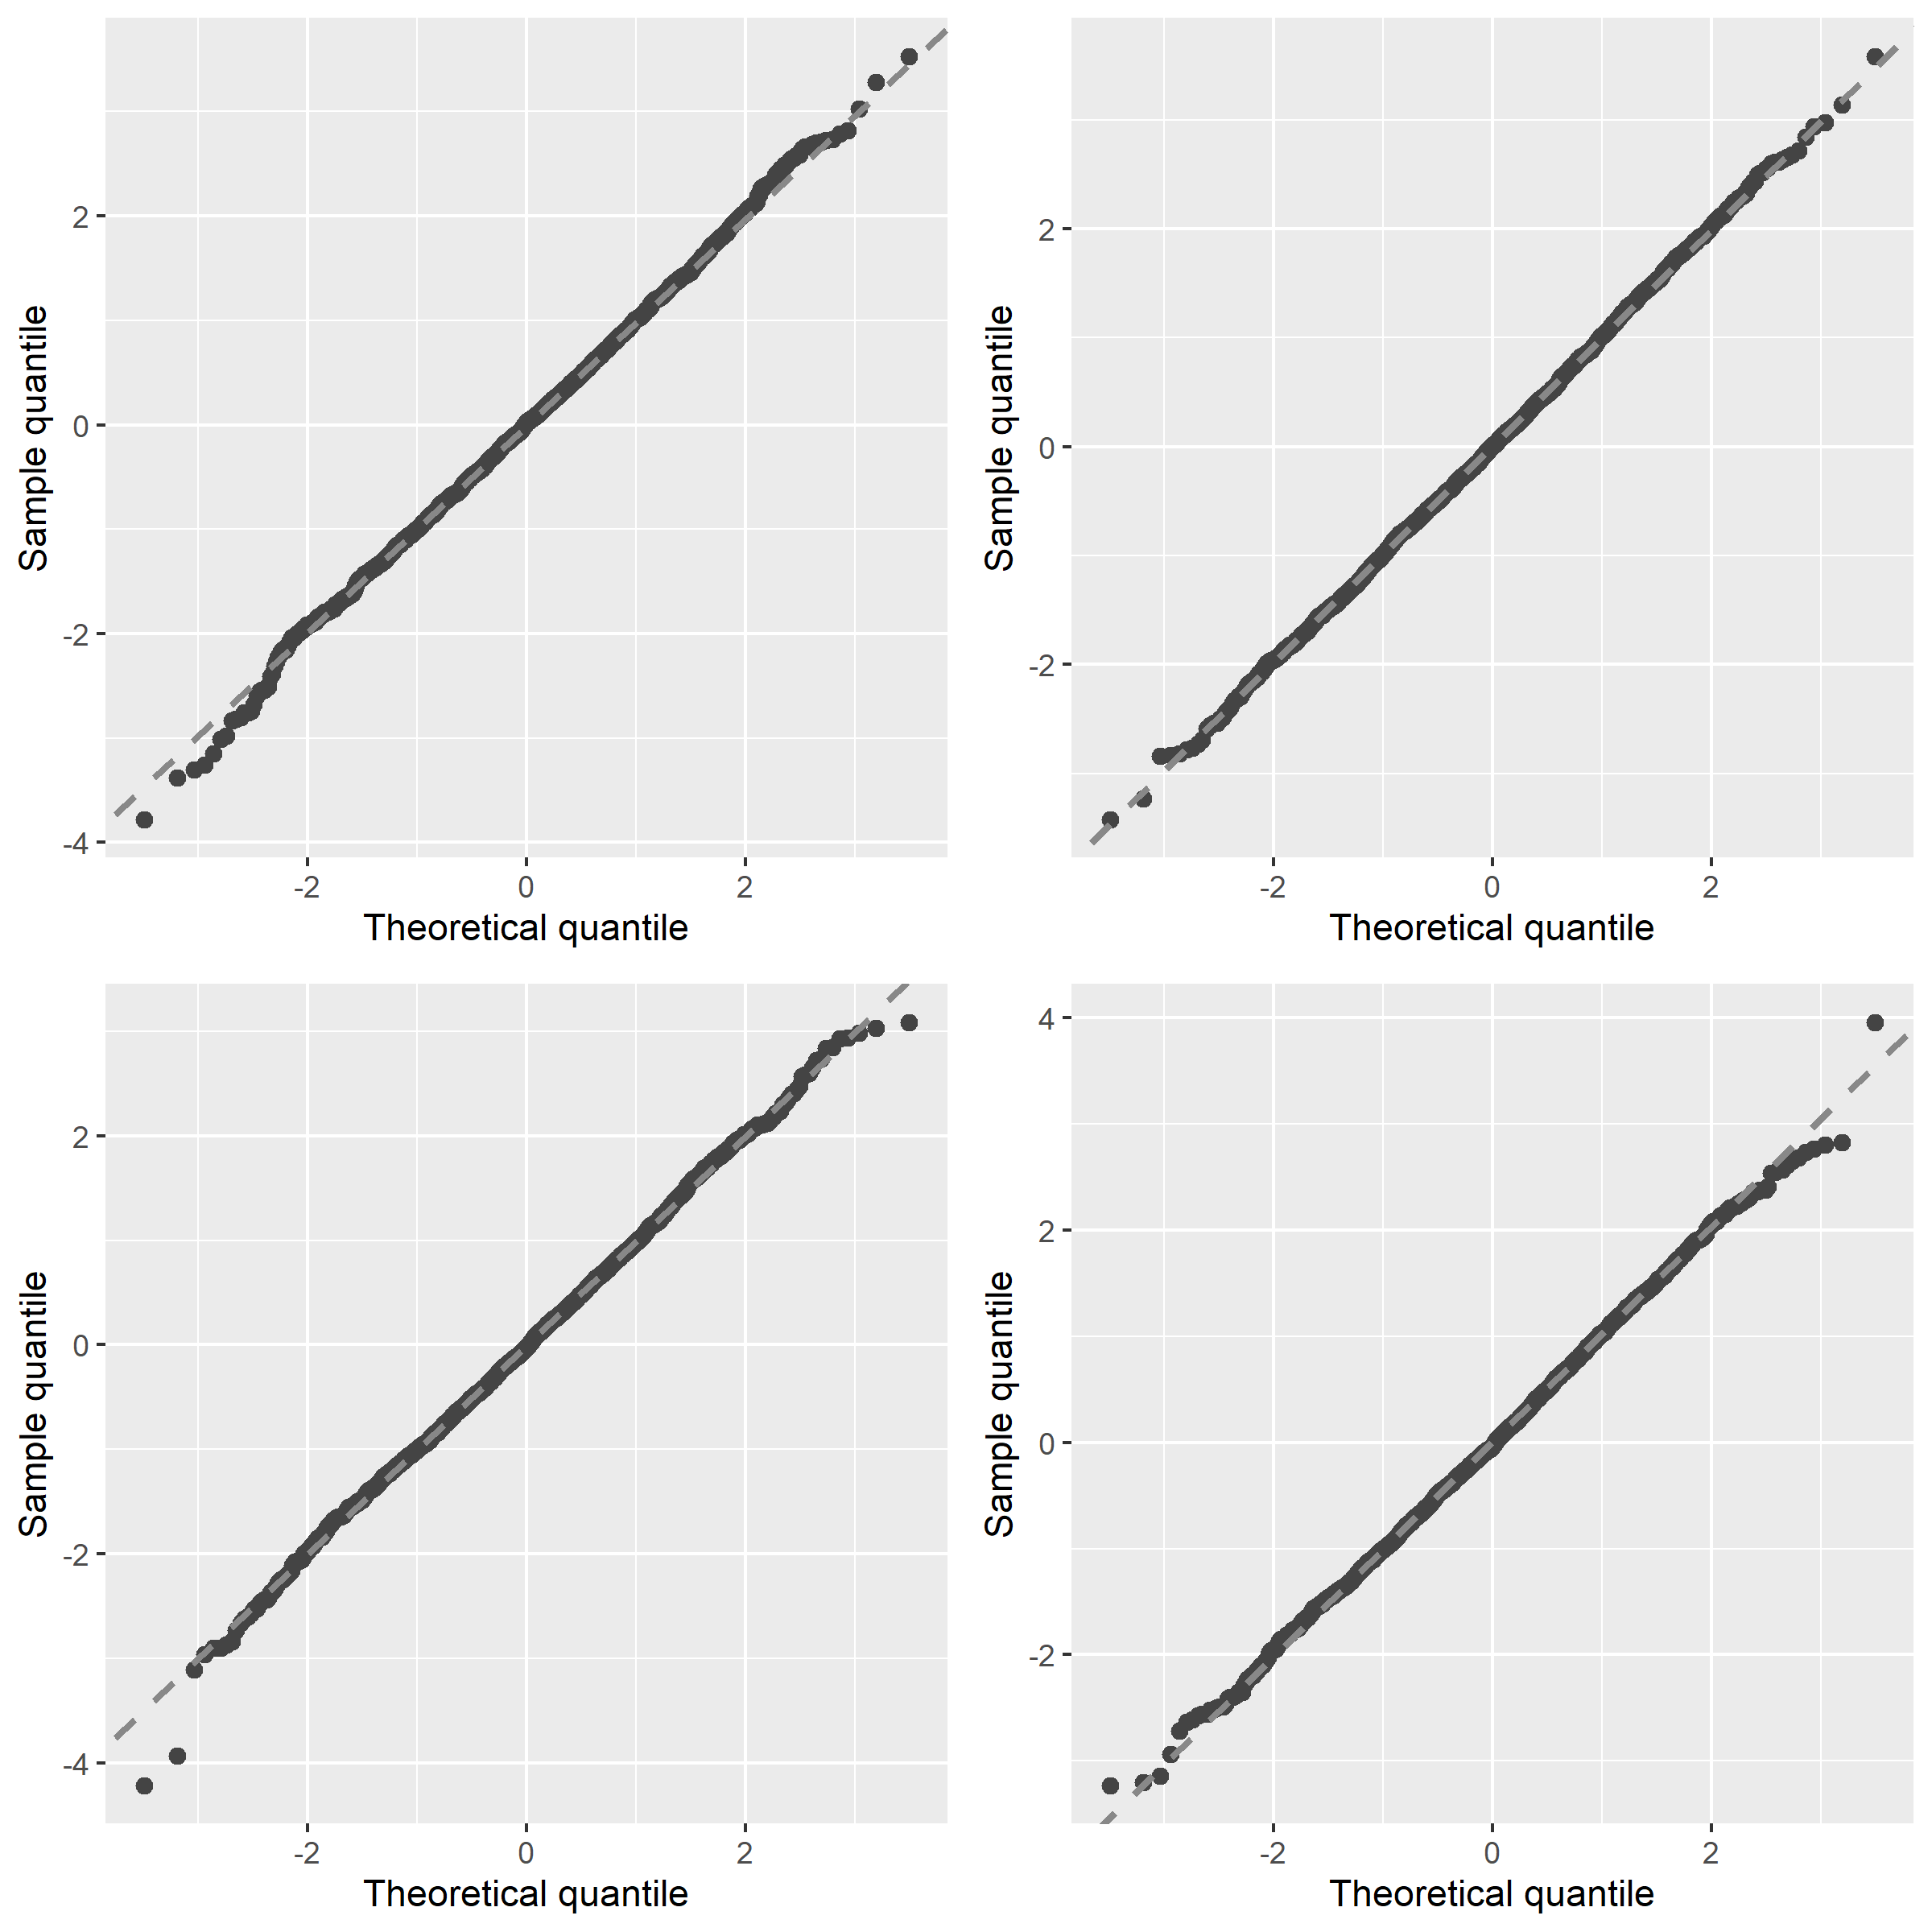
\includegraphics[width=5cm]{fig/qq_12.png} }}%
	\qquad
	\subfloat[\centering 2016]{{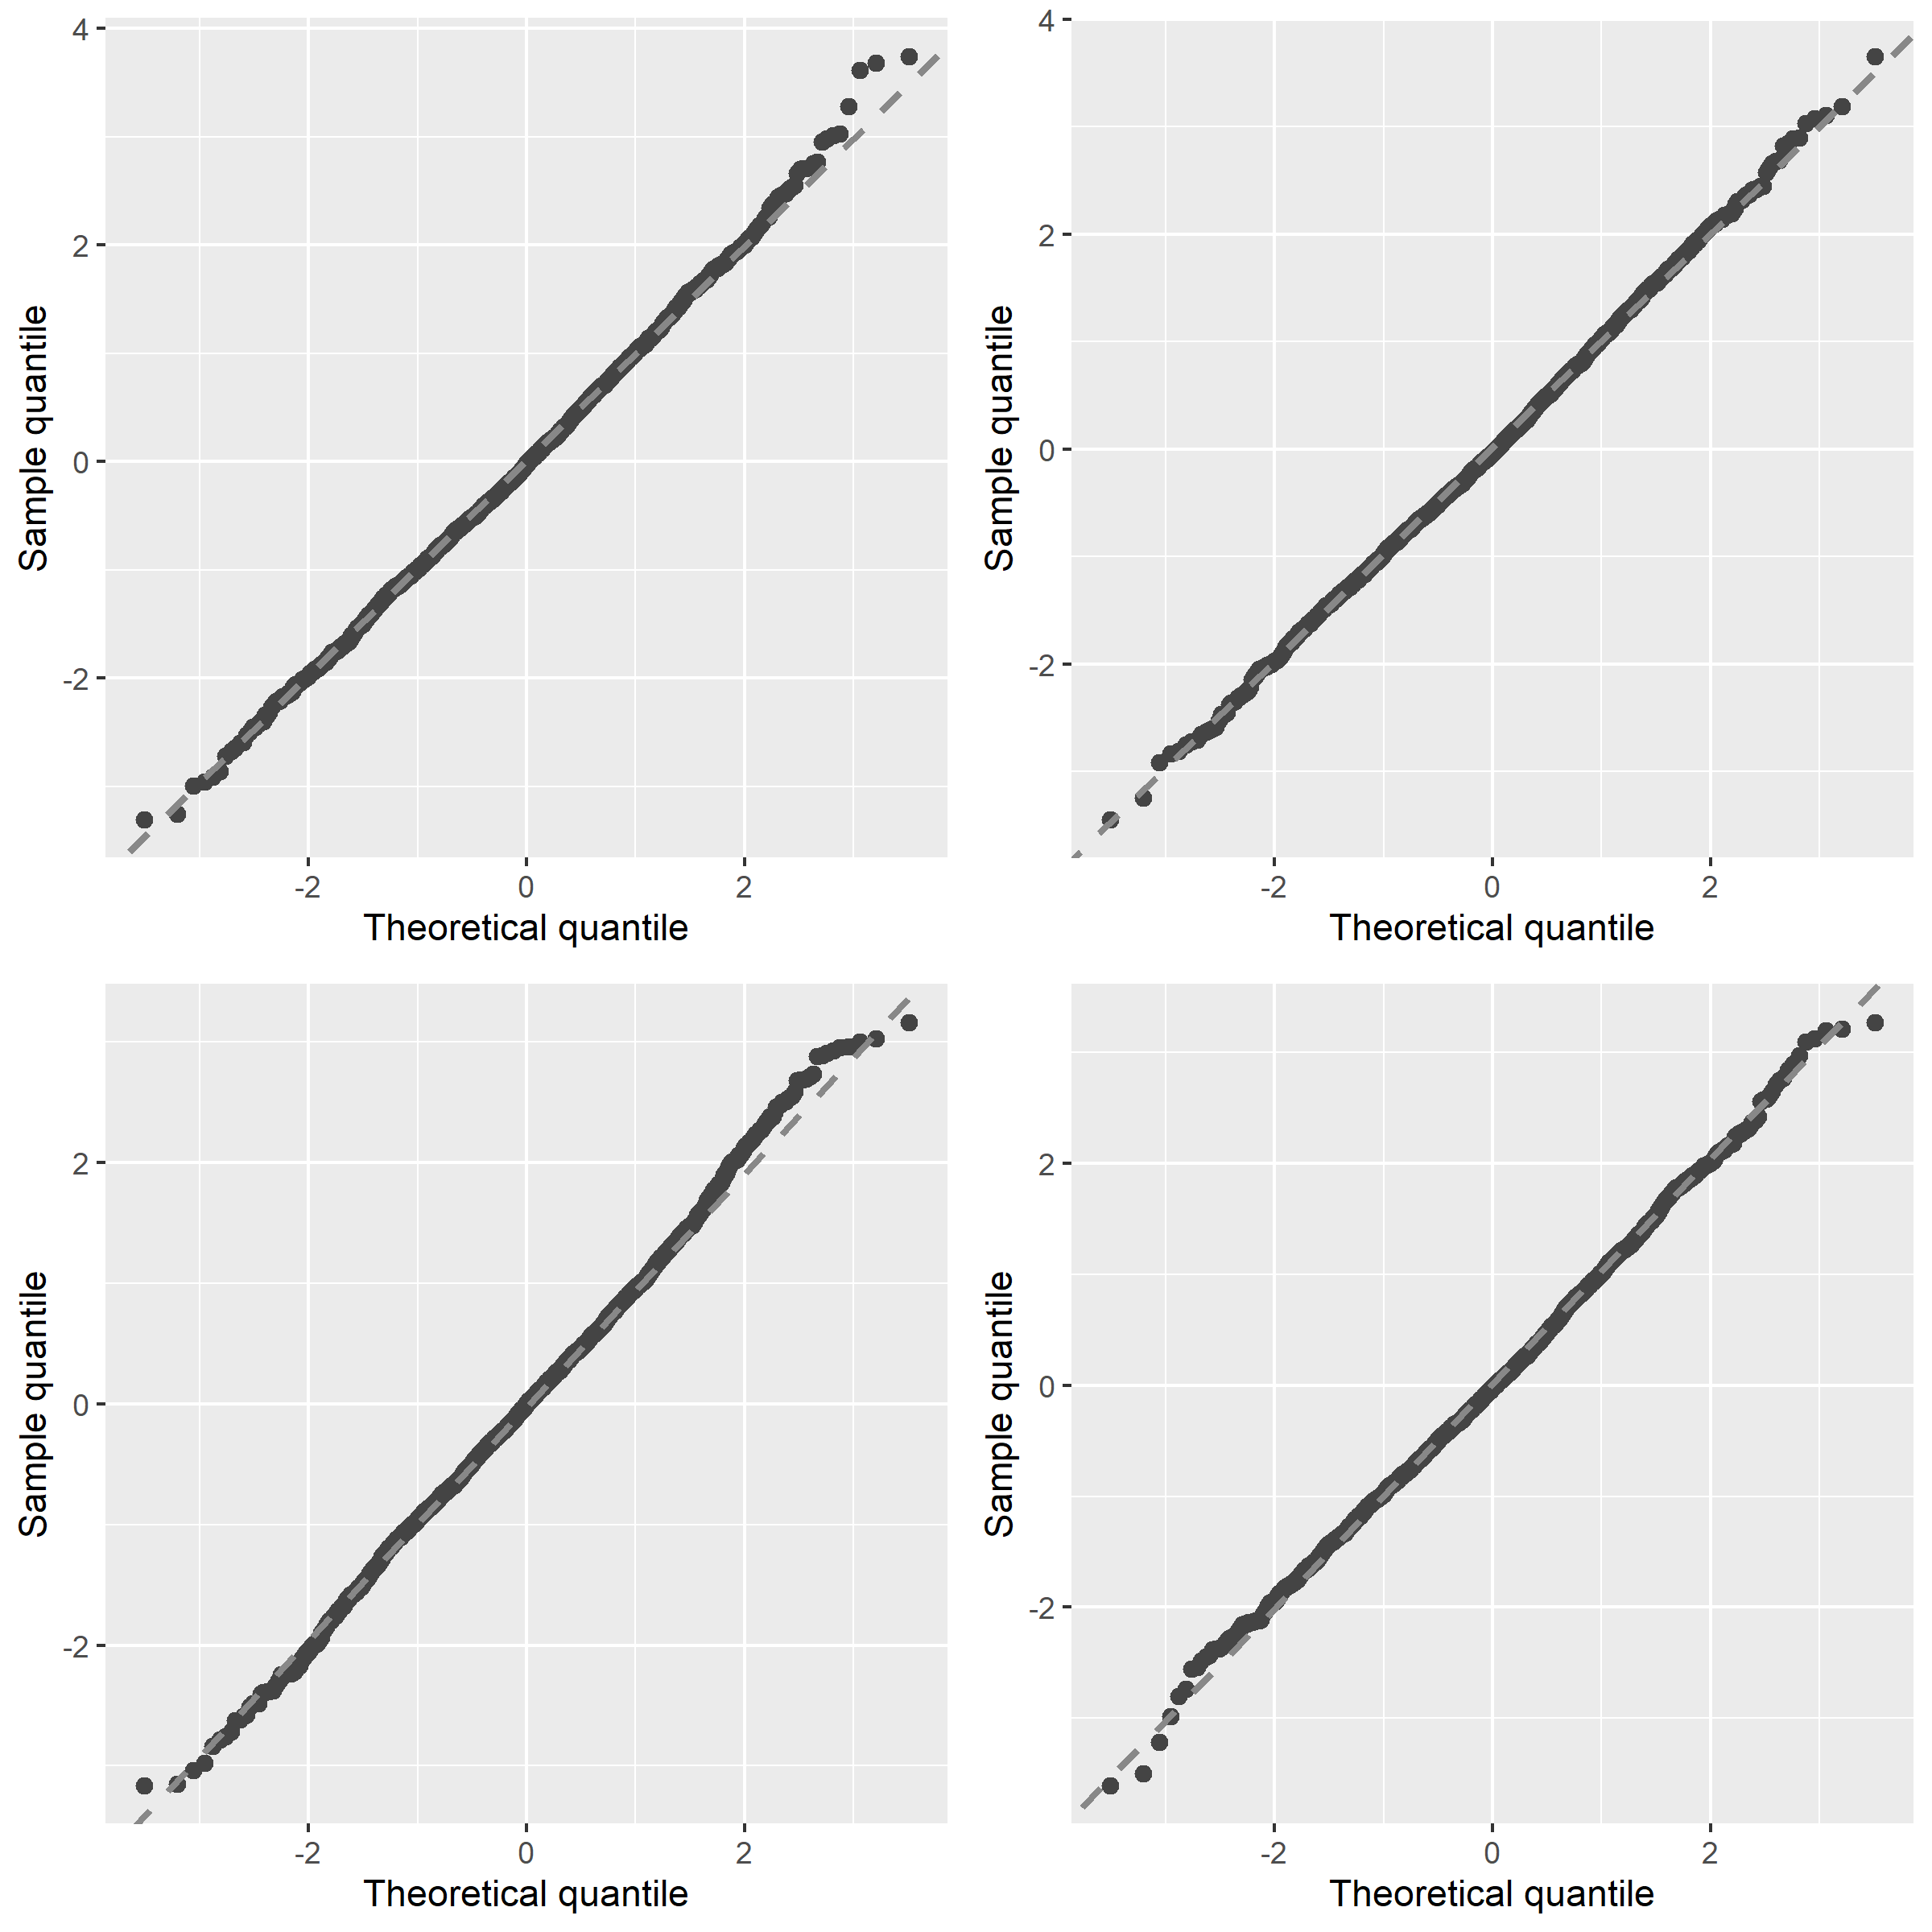
\includegraphics[width=5cm]{fig/qq_16.png} }}%
	\caption{Normal Q-Q Plots for 2012-2016 Ordered Probit Models}%
	\label{qq-2}%
\end{figure}


\section{Discussion}
In this paper, I reconsidered the relationship between political sophistication and causal attributions of black impoverishment in the United States. I argue that advancements in technology, increases in information access, and social movements have created an environment in which obtaining political information is less costly than it once was. Further, scholars and activists have fought to make the public aware of institutional disadvantages faced by black Americans - a message which has been furthered by political elites. Taken together, these trends suggest that a high level of political sophistication need not be necessary for Americans to make structuralist attributions about the causes of black poverty. I replicated the models from \cite{gomez_rethinking_2006} using data from 2012 and 2016 and show that, while sophistication remains negatively related to individualistic attributions, it holds a much weaker relationship with structural attributions than in the late 20th and early 21st Century. In most cases, there is no relationship between the two that is statistically distinguishable from 0 at conventional levels. This may reflect an overall rise in political sophistication; whereas before it required a greater deal of active interest and effort to become politically sophisticated, this process may be much more passive in the 21st Century. Consequently, being able to correctly answer political knowledge questions may no longer indicate individuals with great breadth and depth of knowledge, leading to higher variance in their attributions. Future work should consider ways to measure the political knowledge and interest in such a way as to better elicit the breadth and depth of these characteristics in an information-saturated environment.


\pagebreak
\singlespacing
\bibliography{rethink}


\end{document}
